%%%%%%%%%%%%%%%%%%%%%%%%%%%%%%%%%%%%%%%%%
% Masters/Doctoral Thesis 
% LaTeX Template
% Version 2.3 (25/3/16)
%
% This template has been downloaded from:
% http://www.LaTeXTemplates.com
%
% Version 2.x major modifications by:
% Vel (vel@latextemplates.com)
%
% This template is based on a template by:
% Steve Gunn (http://users.ecs.soton.ac.uk/srg/softwaretools/document/templates/)
% Sunil Patel (http://www.sunilpatel.co.uk/thesis-template/)
%
% Template license:
% CC BY-NC-SA 3.0 (http://creativecommons.org/licenses/by-nc-sa/3.0/)
%
%%%%%%%%%%%%%%%%%%%%%%%%%%%%%%%%%%%%%%%%%

%----------------------------------------------------------------------------------------
%	PACKAGES AND OTHER DOCUMENT CONFIGURATIONS
%----------------------------------------------------------------------------------------

\documentclass[
11pt, % The default document font size, options: 10pt, 11pt, 12pt
%oneside, % Two side (alternating margins) for binding by default, uncomment to switch to one side
%chapterinoneline,% Have the chapter title next to the number in one single line
%english, % ngerman for German
spanish,
singlespacing, % Single line spacing, alternatives: onehalfspacing or doublespacing
%draft, % Uncomment to enable draft mode (no pictures, no links, overfull hboxes indicated)
%nolistspacing, % If the document is onehalfspacing or doublespacing, uncomment this to set spacing in lists to single
%liststotoc, % Uncomment to add the list of figures/tables/etc to the table of contents
%toctotoc, % Uncomment to add the main table of contents to the table of contents
parskip, % Uncomment to add space between paragraphs
%nohyperref, % Uncomment to not load the hyperref package
headsepline, % Uncomment to get a line under the header
]{MastersDoctoralThesis} % The class file specifying the document structure



%----------------------------------------------------------------------------------------
%	INFORMACIÓN DE LA MEMORIA
%----------------------------------------------------------------------------------------

\thesistitle{Monitor para medidores de energía eléctrica} % El títulos de la memoria, se usa en la carátula y se puede usar el cualquier lugar del documento con el comando \ttitle
\degree{Especialista en Sistemas Embebidos } % Nombre del grado, se usa en la carátula y se puede usar el cualquier lugar del documento con el comando \degreename
\author{Ing. Mauricio Barroso Benavides} % Tu nombre, se usa en la carátula y se puede usar el cualquier lugar del documento con el comando \authorname
\supervisor{Mg. Ing. Gonzalo Sanchez (F.A.A.)} % El nombre del director, se usa en la carátula y se puede usar el cualquier lugar del documento con el comando \supname
\juradoUNO{Mg. Ing. Martín Nicolás Menéndez (pertenencia)} % Nombre y pertenencia del un jurado se usa en la carátula y se puede usar el cualquier lugar del documento con el comando \jur1name
\juradoDOS{Mg. Ing. Christian Yañez Flores (pertenencia)} % Nombre y pertenencia del un jurado se usa en la carátula y se puede usar el cualquier lugar del documento con el comando \jur2name
\juradoTRES{Esp. Ing. Esteban Daniel Volentini (pertenencia)} % Nombre y pertenencia del un jurado se usa en la carátula y se puede usar el cualquier lugar del documento con el comando \jur3name
\fechaINICIO{agosto de 2019}
\fechaFINAL{agosto de 2020}

\subject{Memoria del Trabajo Final de la Carrera de Especialización en Sistemas Embebidos de la UBA} % Your subject area, this is not currently used anywhere in the template, print it elsewhere with \subjectname
\keywords{Sistemas Embebidos, CESE, FIUBA} % Keywords for your thesis, this is not currently used anywhere in the template, print it elsewhere with \keywordnames
\university{Universidad de Buenos Aires} % Your university's name and URL, this is used in the title page and abstract, print it elsewhere with \univname
\faculty{{Facultad de Ingeniería}} % Your faculty's name and URL, this is used in the title page and abstract, print it elsewhere with \facname
\department{Departamento de Electrónica} % Your department's name and URL, this is used in the title page and abstract, print it elsewhere with \deptname
\group{{Laboratorio de Sistemas Embebidos}} % Your research group's name and URL, this is used in the title page, print it elsewhere with \groupname


%\hypersetup{pdftitle=\ttitle} % Set the PDF's title to your title
%\hypersetup{pdfauthor=\authorname} % Set the PDF's author to your name
%\hypersetup{pdfkeywords=\keywordnames} % Set the PDF's keywords to your keywords


%\newcaptionname{spanish}{\acknowledgementname}{Agradecimientos}
%\newcaptionname{spanish}{\authorshipname}{Declaración de Autoría}
%\newcaptionname{spanish}{\abbrevname}{Glosario}
%\newcaptionname{spanish}{\byname}{por}
%
%\renewcommand{\lstlistingname}{Código}% Listing -> Algorithm
%\renewcommand{\lstlistlistingname}{Índice de \lstlistingname s}% List of Listings -> List of Algorithms
%
%\renewcommand{\listtablename}{Índice de Tablas}
%\renewcommand{\tablename}{Tabla} 

\addtolength{\footnotesep}{1mm} % Espacio adicional en los footnotes

\begin{document}

\frontmatter % Use roman page numbering style (i, ii, iii, iv...) for the pre-content pages

\pagestyle{plain} % Default to the plain heading style until the thesis style is called for the body content

%----------------------------------------------------------------------------------------
%	CARÁTULA
%----------------------------------------------------------------------------------------

\begin{titlepage}
\begin{center}



\includegraphics[width=.8\textwidth]{./Figures/logoFIUBA.png}
\vspace{2cm}

\textsc{\huge{Carrera de Especialización en\\ \vspace{5px} Sistemas Embebidos}}
\vspace{.5cm} % Thesis type

\textsc{\Large Memoria del Trabajo Final}\\[1cm] % Thesis type
%\vspace{1.5cm}
{\huge \bfseries \ttitle\par}\vspace{0.4cm} % Thesis title

\vfill

\vspace{2cm}
\LARGE\textbf{Autor:\\
\authorname}\\ % Author name

\vspace{1.5cm}

\large
{Director:} \\
{\supname} % Supervisor name
 
\vspace{1cm}
Jurados:\\	
\jurunoname\\
\jurdosname\\
\jurtresname

\vspace{1cm}

\textit{Este trabajo fue realizado en la Ciudad de Salta,\\ entre \fechaINICIOname \hspace{1px} y \fechaFINALname.}
\end{center}
\end{titlepage}


%----------------------------------------------------------------------------------------
%	RESUMEN - ABSTRACT 
%----------------------------------------------------------------------------------------

\begin{abstract}
\addchaptertocentry{\abstractname} % Add the abstract to the table of contents
%
%The Thesis Abstract is written here (and usually kept to just this page). The page is kept centered vertically so can expand into the blank space above the title too\ldots
\centering

La presente memoria tiene como objetivo describir el desarrollo de un dispositivo electrónico, capaz de monitorear la información de consumo de energía eléctrica proveniente de medidores de uso domiciliario. El trabajo fue propuesto por la cooperativa de servicios eléctricos de la ciudad boliviana de Tupiza, COPELECT, para automatizar la lectura de los medidores que tiene instalados en los hogares de sus más de diez mil abonados.

En la elaboración de este trabajo se ven plasmados los conocimientos adquiridos en la carrera de especialización, sobre ingeniería de software, sistemas operativos en tiempo real I y II, protocolos de comunicación y diseño de circuitos impresos.

\end{abstract}

%----------------------------------------------------------------------------------------
%	CONTENIDO DE LA MEMORIA  - AGRADECIMIENTOS
%----------------------------------------------------------------------------------------

\begin{acknowledgements}
%\addchaptertocentry{\acknowledgementname} % Descomentando esta línea se puede agregar los agradecimientos al índice
\vspace{1.5cm}

Esta sección es para agradecimientos personales y es totalmente \textbf{OPCIONAL}.  

\end{acknowledgements}

%----------------------------------------------------------------------------------------
%	LISTA DE CONTENIDOS/FIGURAS/TABLAS
%----------------------------------------------------------------------------------------
\renewcommand{\listtablename}{Índice de Tablas} %TODO eliminar esta línea

\tableofcontents % Prints the main table of contents
%
\listoffigures % Prints the list of figures
%
\listoftables % Prints the list of tables


%----------------------------------------------------------------------------------------
%	CONTENIDO DE LA MEMORIA  - DEDICATORIA
%----------------------------------------------------------------------------------------

\dedicatory{\textbf{Dedicado a... [OPCIONAL]}}  % escribir acá si se desea una dedicatoria

%----------------------------------------------------------------------------------------
%	CONTENIDO DE LA MEMORIA  - CAPÍTULOS
%----------------------------------------------------------------------------------------

\mainmatter % Begin numeric (1,2,3...) page numbering

\pagestyle{thesis} % Return the page headers back to the "thesis" style

%\renewcommand{\tablename}{Tabla} %TODO eliminar esta línea

% Incluir los capítulos como archivos separados desde la carpeta Chapters
% Descomentar las líneas a medida que se escriben los capítulos

% Chapter 1

\chapter{Introducción General} % Main chapter title

\label{Chapter1} % For referencing the chapter elsewhere, use \ref{Chapter1} 
\label{IntroGeneral}

%----------------------------------------------------------------------------------------

% Define some commands to keep the formatting separated from the content 
\newcommand{\keyword}[1]{\textbf{#1}}
\newcommand{\tabhead}[1]{\textbf{#1}}
\newcommand{\code}[1]{\texttt{#1}}
\newcommand{\file}[1]{\texttt{\bfseries#1}}
\newcommand{\option}[1]{\texttt{\itshape#1}}
\newcommand{\grados}{$^{\circ}$}

%----------------------------------------------------------------------------------------

%\section{Introducción}

En este capítulo se presenta una descripción del proceso que COPELECT realiza para obtener información sobre el consumo eléctrico de sus abonados, nociones sobre medidores inteligentes, una comparación de las soluciones comercialmente disponibles en esta temática, las razones que motivaron al desarrollo del trabajo junto con sus objetivos y alcances.

%----------------------------------------------------------------------------------------

\section{Medición del consumo eléctrico domiciliario}

En los hogares se dispone de diversos dispositivos eléctricos y electrónicos que son utilizados para entretenimiento, labores domésticas, trabajo, etc. La energía eléctrica consumida por estos dispositivos es medida en vatio-hora, simbolizado Wh \citep{WEBSITE:1}. El kWh, equivalente a 1000 vatios-hora, se utiliza para la facturación del consumo de energía eléctrica por parte de las compañías prestadoras del servicio \citep{WEBSITE:1}. Para este fin, las compañías instalan en los hogares de sus abonados dispositivos llamados medidores, que se encargan de contar la cantidad de kWh consumidos. También, los medidores proporcionan una interfaz para que los funcionarios de dichas compañías puedan registrar la información de consumo eléctrico.

Las mayor parte de compañías prestadoras del servicio eléctrico utilizan principalmente dos tipos de medidores para medir el consumo eléctrico domiciliario. Estos son:

\begin{enumerate}
	\item Medidores analógicos: contienen un disco giratorio metálico y un contador analógico que indica el total de kWh consumidos. Cuando la corriente fluye a través del medidor, se genera un campo eléctrico que impulsa el disco a girar. Entonces, la velocidad angular del disco está relacionada linealmente con el consumo eléctrico. Cada medidor analógico tiene un valor que indica el número de revoluciones que representan exactamente 1 kWh \citep{WEBSITE:2}.
	\item Medidores digitales: tienen una interfaz que consiste en una pequeña pantalla digital para mostrar la cantidad total de kWh consumidos y una salida de pulso óptico compuesta por un LED (\textit{Light-Emitting Diode}). Cada cierta cantidad de transiciones entre el estado apagado y encendido del LED representa exactamente 1 kWh consumido, esta cantidad es una constante indicada por el medidor como impulsos/kWh. Por lo tanto, monitorear el parpadeo del LED brinda la capacidad obtener el consumo eléctrico en el tiempo. El valor de los impulsos/kWh difiere según el fabricante del medidor y generalmente se encuentra debajo del LED \citep{WEBSITE:2}.
\end{enumerate}

En las figuras 1.1 y 1.2, se pueden observar un medidor de consumo eléctrico analógico y otro digital, respectivamente.

\begin{figure}[h]
	\centering
	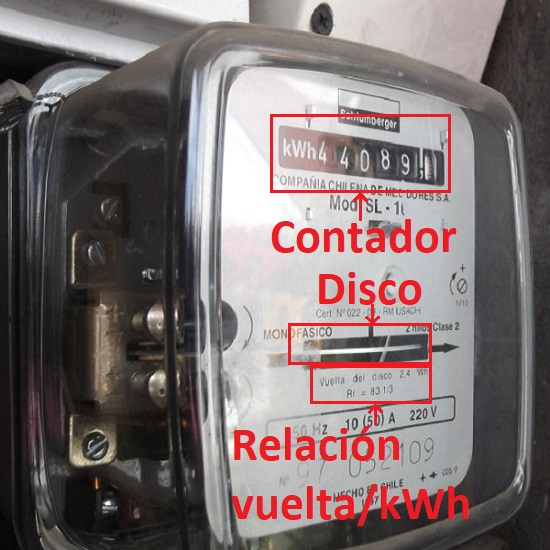
\includegraphics[scale=0.35]{./Figures/analog_meter.jpg}
	\caption{ Medidor de consumo eléctrico analógico.}
	\label{fig:cuadradoAzul}
\end{figure}

\begin{figure}[h]
	\centering
	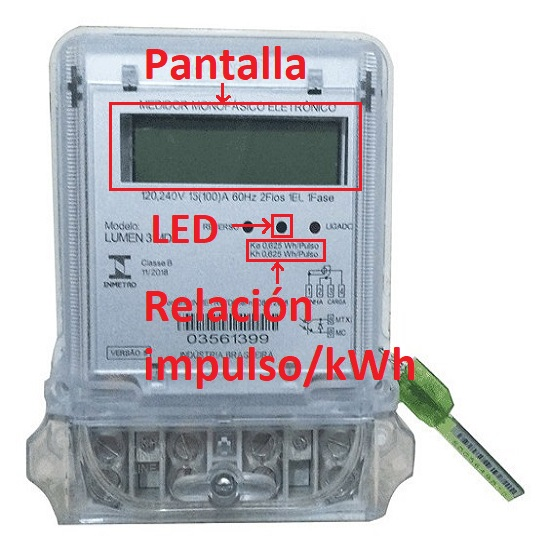
\includegraphics[scale=0.55]{./Figures/digital_meter.jpg}
	\caption{ Medidor de consumo eléctrico digital.}
	\label{fig:cuadradoAzul}
\end{figure}

Cuando la compañía prestadora del servicio eléctrico quiere obtener la información de consumo de sus medidores, lo hace registrando el valor que exhibe la interfaz del medidor, que posee un contador analógico en el caso de un medidor analógico o una pantalla digital en el caso de un medidor digital, ambas exhiben el total de kWh consumidos por el abonado.

La cooperativa de servicios eléctricos Tupiza Ltda., COPELECT, de la ciudad de Tupiza, Bolivia, tiene instalados alrededor de diez mil medidores de consumo eléctrico analógicos y digitales de uso domiciliario en los hogares de sus abonados, que son monitoreados para determinar el consumo eléctrico de cada uno de ellos. El monitoreo lo realizan funcionarios que se desplazan por toda la ciudad y registran el valor que exhibe la interfaz de los medidores junto con el nombre del abonado al que corresponde. Esta información es recopilada y utilizada para emitir la factura correspondiente de cada abonado. Finalmente, la factura emitida es impresa y llevada por los funcionarios a los hogares de los abonados para que tengan conocimiento del monto que deben pagar por su consumo eléctrico.

El proceso de monitoreo antes descrito es llevado a cabo una vez al mes por doce funcionarios, quienes tardan alrededor de ocho días en registrar toda la información de los medidores. Posteriormente, esa información es introducida a una base de datos que funciona en un servidor local ubicado en las oficinas centrales de COPELECT. La cantidad de kWh consumidos que deben ser facturados se determinan al restar el conteo de kWh del mes anterior con el actual. En casos particulares donde los funcionarios no pueden acceder al medidor para registrar el conteo de kWh consumidos, se emite la factura con los datos del mes anterior.

%----------------------------------------------------------------------------------------

\section{Medición inteligente}

La mayoría de los medidores de consumo eléctrico utilizados por parte de las compañías que prestan dicho servicio, sean estos analógicos o digitales, son dispositivos cuya única función es medir y exhibir mediante su interfaz la cantidad de kWh consumidos. Esta información únicamente es útil para la compañía y no brinda otros datos de relevancia. Existen también en el mercado otro tipo de medidores cuyas prestaciones son beneficiosas tanto para la compañía como para el abonado.

Los medidores inteligentes o \textit{smart meters}, son dispositivos que graban información como el consumo eléctrico, niveles de voltaje, corriente y factor de potencia. Esta información es comunicada a la compañía eléctrica para generar la facturación de sus servicios y a los abonados para que tengan mayor conocimiento sobre el comportamiento de su consumo eléctrico. Los smart meters típicamente graban la información eléctrica en tiempo real o en intervalos cortos a lo largo del día.

En la figura 1.3 se observa un smart meter.

\begin{figure}[h]
	\centering
	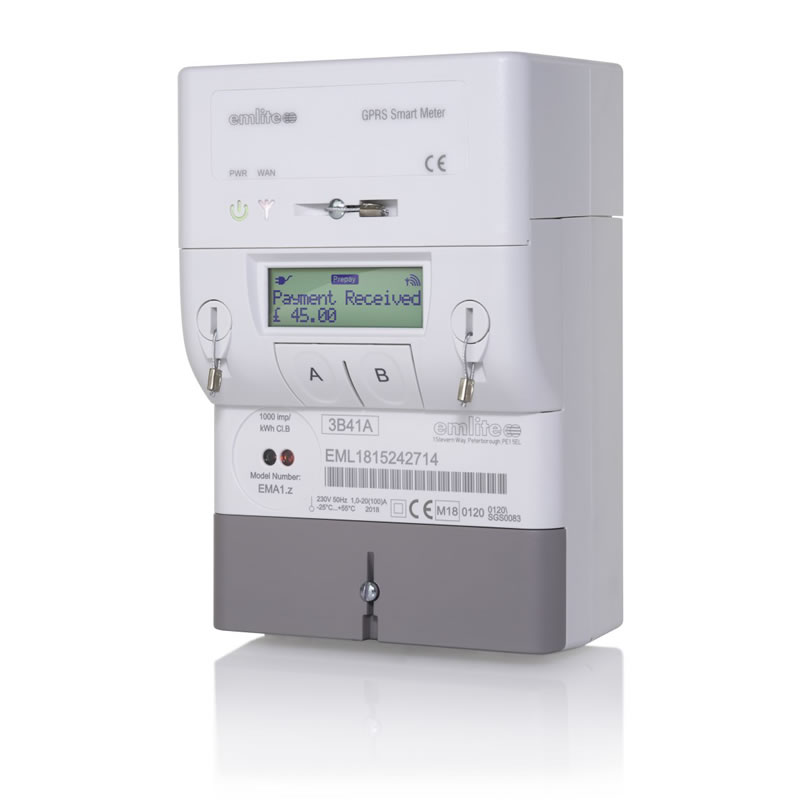
\includegraphics[scale=0.29]{./Figures/smart_meter.jpg}
	\caption{Smart meter de la firma emlite\protect\footnotemark.}
	\label{fig:cuadradoAzul}
\end{figure}

\footnotetext{Imagen tomada de: \url{https://www.jwsmartmeters.co.uk/brand/emlite/}}

Para mejorar el proceso de monitoreo y adquisición de información sobre consumo eléctrico, los smart meters representan una solución idónea, pero, el costo de su implementación los vuelve inviables para muchas compañías que ofrecen el servicio eléctrico. Entonces, debido a la problemática antes planteada, existe un mercado creciente para medidores no inteligentes, ampliados con un dispositivo que transfiere la información sobre el consumo eléctrico a la compañía y al abonado.

El dispositivo añadido a los medidores eléctricos de uso convencional puede utilizar distintos tipos de sensores para obtener la información de consumo eléctrico. Estos son:

\begin{itemize}
	\item Pinza de corriente: es una bobina sujeta alrededor de un conductor eléctrico. Cuando la corriente pasa a través del conductor, se genera un campo eléctrico. La bobina medirá este campo eléctrico y lo traducirá  a un flujo de corriente \citep{WEBSITE:3}.
	\item Cámara: podría ser situada en frente de del medidor y periódicamente tomar obtener fotografías del contador o pantalla. Las lecturas del consumo pueden ser extraídas de estas fotografías con técnicas de procesamiento de imágenes \citep{ARTICLE:1}.
	\item Foto-reflector: consiste en un LED y un fototransistor en una sola carcasa. Este sensor es posicionado en frente del disco que poseen los medidores analógicos, cuando el LED emite luz es reflejada por el disco y medida por el fototransistor \citep{WEBSITE:4}.
	\item Fototransistor: en conjunto con la salida de pulso óptico de los medidores digitales, se puede contar la cantidad de veces que el LED pasa de estado bajo a alto, para determinar el consumo eléctrico \citep{WEBSITE:5}.
\end{itemize}

%----------------------------------------------------------------------------------------

\section{Soluciones disponibles en el mercado}

Como se mencionó en la subsección anterior, dotar a los medidores convencionales de un dispositivo que amplíe sus funciones, es una manera de mejorar el proceso de monitoreo y adquisición de información de consumo eléctrico que realizan las compañías prestadoras de servicio.

Comercialmente existen dispositivos que cumplen esta función y utilizan alguno de los sensores adecuados para este fin. La fabricación de estos dispositivos se realiza sobre todo en Estados Unidos y algunos países europeos. A continuación se listan algunos dispositivos que utilizan la salida de pulso óptico de los medidores digitales para registrar el consumo de kWh:

\begin{itemize}
	\item PA-FL \citep{WEBSITE:6} es un contador de pulsos con comunicación inalámbrica de la firma SyxthSense. Es alimentado mediante baterías o una fuente de tensión de 24 V y trabaja como parte de un sistema propietario de SyxthSense. Puede ser instalado en medidores de electricidad, agua o gas y transmitir inalámbricamente los datos que registra utilizando una modulacion de tipo FSK (\textit{Frequency Shift Keying}) en la banda de 868.3 MHz. También, posee dos salidas de potencia de 1 A y y 60 V que pueden ser utilizadas para interactuar con otros dispositivos eléctrico o electrónicos. Dispone de una carcasa con certificación IP54. En la figura 1.4 se muestra una fotografía del dispositivo.
	
	\begin{figure}[h]
		\centering
		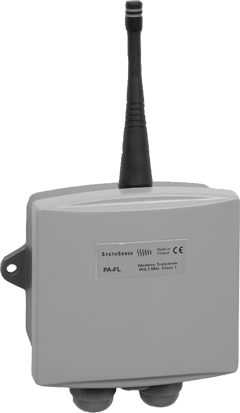
\includegraphics[scale=0.47]{./Figures/PA-FL.png}
		\caption{Registrador de pulsos PA-FL de la firma SyxthSense\protect\footnotemark.}
		\label{fig:cuadradoAzul}
	\end{figure}
	
	\footnotetext{Imagen tomada de: \citep{WEBSITE:6}}

	\item AirTM-100S \citep{WEBSITE:7}: creado por la firma iNES, es un dispositivo diseñado para adquirir datos de medidores de energía eléctrica, agua y gas. Utiliza la salida de pulso óptico de medidores digitales para registrar el consumo del servicio. Es alimentado por una batería de 3.6 V que le brinda un tiempo de vida de aproximadamente cinco años, tiene carcasa con certificación IP65 y puede transmitir utilizando redes SIGFOX\footnote{SIGFOX. Es un operador de red global que implementa redes inalámbricas para conectar dispositivos de bajo consumo.}  a una frecuencia de 868 MHz. El dispositivo puede observarse en la figura 1.5.
	
	\begin{figure}[h]
		\centering
		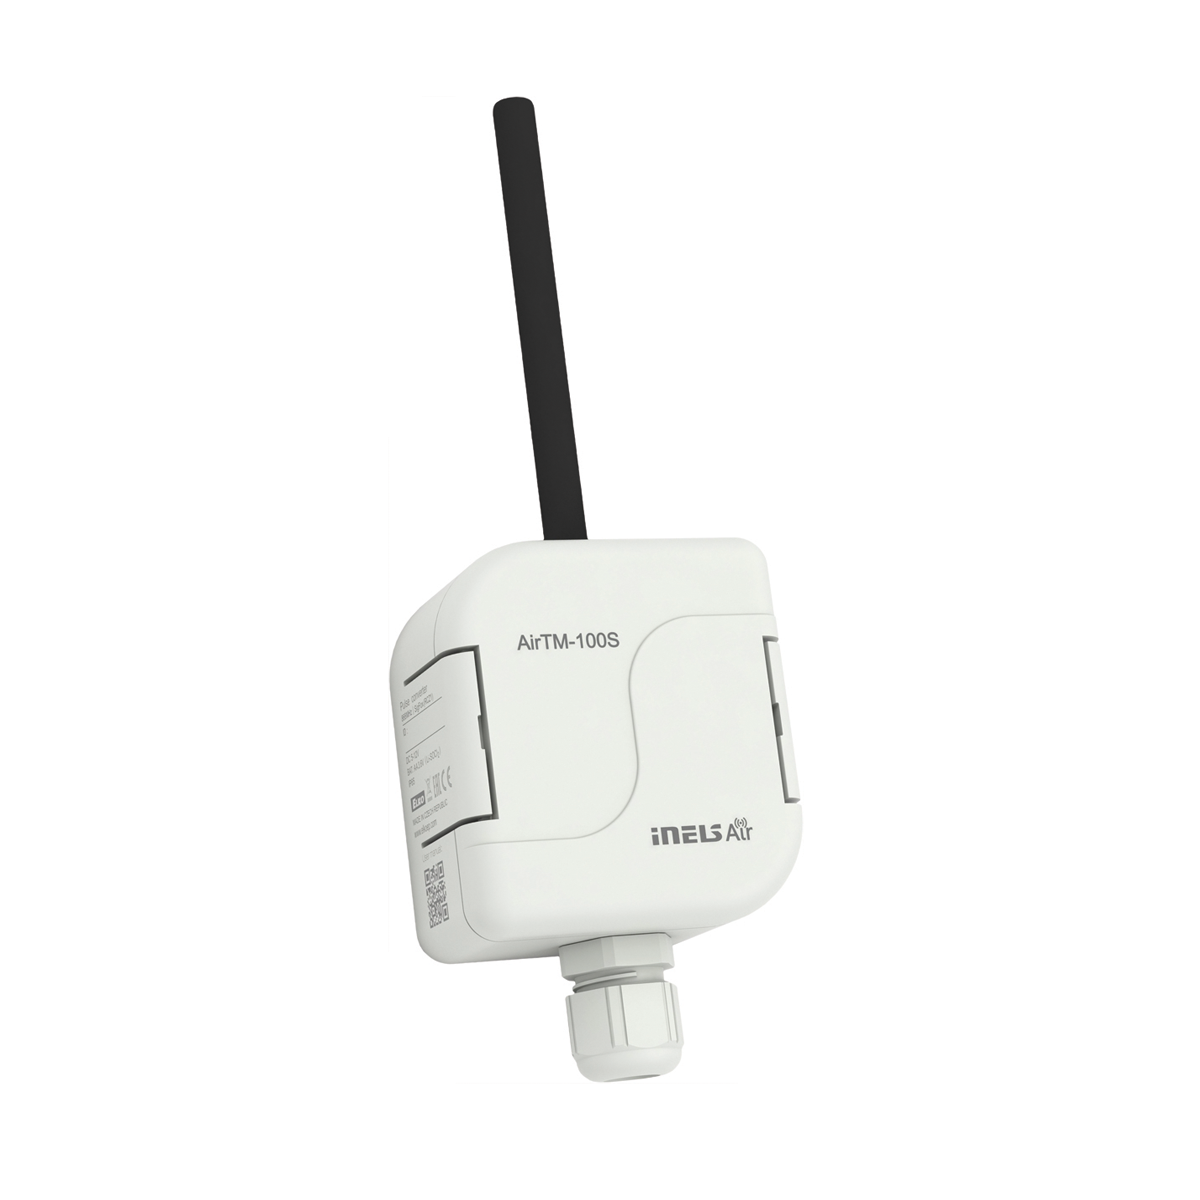
\includegraphics[scale=0.22]{./Figures/airtm-100s.png}
		\caption{Registrador de pulsos AirTM-100S de la firma iNES\protect\footnotemark.}
		\label{fig:cuadradoAzul}
	\end{figure}	
\end{itemize}

\footnotetext{Imagen tomada de: \citep{WEBSITE:7}}

%----------------------------------------------------------------------------------------

\section{Motivación}

Hoy en día, no solo las compañías de servicio eléctrico están interesadas en los números que proporcionan los medidores domiciliarios, sino también los propios abonados. Con la introducción del \textit{smart meter}, la cantidad de electricidad consumida se puede comunicar en tiempo real al abonado. Este consumo se presenta en un dispositivo, por ejemplo, un teléfono inteligente o una tableta, que brinda más información a los abonados y los motiva a reducir su consumo de energía hasta en un 9\% \citep{WEBSITE:8}.Entonces, el trabajo se originó como una propuesta de COPELECT, para contar con una alternativa tecnológica que optimice el proceso de monitoreo de los medidores que tiene instalados en la ciudad boliviana de Tupiza y proporcione a sus usuarios una manera de conocer su consumo eléctrico de manera oportuna.

Otra motivación importante para la realización de este trabajo fue la aplicación de los conocimientos adquiridos en la carrera de Especialización, para desarrollar e implementar un dispositivo basado en buenas prácticas de desarrollo de \textit{firmware} y \textit{hardware}, que sea lo suficientemente robusto y eficiente para que puedan reproducirlo por cientos o miles de unidades.

%----------------------------------------------------------------------------------------

\section{Objetivos y alcance}

El objetivo principal de este trabajo fue desarrollar e implementar un dispositivo electrónico, capaz de monitorear un medidor de consumo eléctrico de uso domiciliario mediante la salida de pulso óptico incorporada, para proporcionar la información obtenida a la compañía prestadora del servicio de manera remota y permitir al abonado conocer su consumo eléctrico en el momento que realiza la consulta a través de una interfaz gráfica web.

El alcance de este proyecto incluye:

\begin{itemize}
	\item Un prototipo comercial que pueda ser instalado en los medidores de consumo eléctrico de COPELECT.
	\item Manual de uso e instalación.
\end{itemize}
\chapter{Introducción Específica} % Main chapter title

\label{Chapter2}

%----------------------------------------------------------------------------------------
%	SECTION 1
%----------------------------------------------------------------------------------------

El presente capítulo presenta los requerimientos del dispositivo, una descripción de los bloques que lo componen y la planificación que se siguió para lograr satisfactoriamente el desarrollo.

%----------------------------------------------------------------------------------------

\section{Requerimientos}

El dispositivo tiene dos tipos de requerimientos, funcionales y no funcionales. Los funcionales, se refieren a la capacidad para cumplir con ciertas tareas impuestas, que garantizan un correcto desempeño del dispositivo en general. Los no funcionales, tienen relación con temas de carácter económico e informativo.

\subsection{Requerimientos funcionales}

\begin{itemize}
	\item El dispositivo deberá poseer conexión Wi-Fi\footnote{Wi-Fi. Es una tecnología inalámbrica para la interconexión de dispositivos electrónicos.}
	\item El dispositivo deberá funcionar como servidor web local.
	\item El dispositivo deberá contar con la hora y fecha exactas.
	\item El dispositivo deberá interpretar los pulsos ópticos provenientes de un medidor de consumo de energía eléctrica domiciliario.
	\item El dispositivo deberá poseer una memoria no volátil para registrar datos como la hora, fecha, conteo de pulsos e ID del usuario; durante al menos tres meses.
	\item El dispositivo deberá contar con un sistema de adquisición, procesamiento, transmisión y recepción de datos, el mismo podrá ser implementado en un microcontrolador con Wi-Fi integrado.
	\item El dispositivo deberá poseer una interfaz web para que los usuarios puedan observar un registro histórico de su consumo de energía eléctrica.
	\item El dispositivo deberá poder establecer conexión con un gateway LoRa, para enviar diariamente en formato hexadecimal la hora, fecha, consumo de energía eléctrica e ID del usuario.
\end{itemize}

\subsection{Requerimientos no funcionales}

\begin{itemize}
	\item El dispositivo deberá tener un precio menor a 50 \$us.
	\item El dispositivo deberá contar con manuales de uso e instalación.
\end{itemize}

%----------------------------------------------------------------------------------------

\section{Esquema general del sistema}

Para cumplir con todos los requerimientos funcionales expuestos en la sección anterior, los componentes mínimos necesarios y su interconexión se muestran en el diagrama en bloques de la figura 2.1.

\begin{figure}[h]
	\centering
	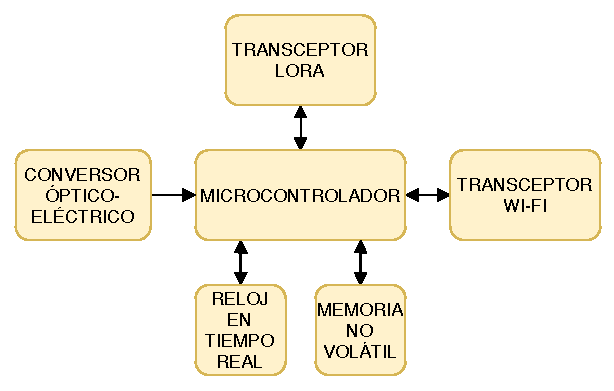
\includegraphics[scale=1.2]{./Figures/general_blocks.pdf}
	\caption{Diagrama en bloques general del dispositivo.}
	\label{fig:cuadradoAzul}
\end{figure}

En el diagrama anterior, el conversor óptico-eléctrico, transforma los pulsos de luz provenientes del LED de un  medidor de consumo eléctrico a pulsos eléctricos y los entrega al microcontrolador. El microcontrolador procesa estos pulsos y realiza el cálculo del consumo eléctrico, esa información junto con la hora y fecha provenientes del reloj en tiempo real, son almacenados en la memoria no volátil para su posterior utilización. El transceptor Wi-Fi, se comunica con el microcontrolador para obtener los datos que serán utilizados para generar la interfaz gráfica mostrada al usuario. El transceptor LoRa, tiene la función de establecer comunicación bidireccional con un dispositivo concentrador LoRa, para enviar la información de la memoria no volátil y recibir parámetros de funcionamiento.

\subsection{Conversor óptico-eléctrico}

Es el encargado de convertir la salida de pulso óptico de medidores eléctricos digitales a pulsos eléctricos, para que puedan ser interpretados por un microcontrolador. Esta información determina el consumo eléctrico que registra el medidor.

La salida de pulso óptico de los medidores eléctricos digitales, esta compuesta por un LED de color rojo, que emite luz cuando se ha consumido una cierta cantidad de kWh. El valor de la relación entre los pulsos emitidos y el consumo eléctrico, es un parámetro intrínseco del medidor, que varía según el modelo y la firma que lo fabrica.

Para realizar la conversión de pulsos de luz a pulsos eléctricos, existen principalmente dos transductores que cumplen cabalmente esta función:

\begin{itemize}
	\item Fotoresistencia: es una resistencia cuyo valor se modifica en función a la intensidad de luz incidente. También es conocida como LDR (\textit{Light-Dependent Resistor}, resistencia dependiente de la luz) \citep{BOOK:2}. En la figura 2.2 se observa una fotoresistencia.
	
	\begin{figure}[h]
		\centering
		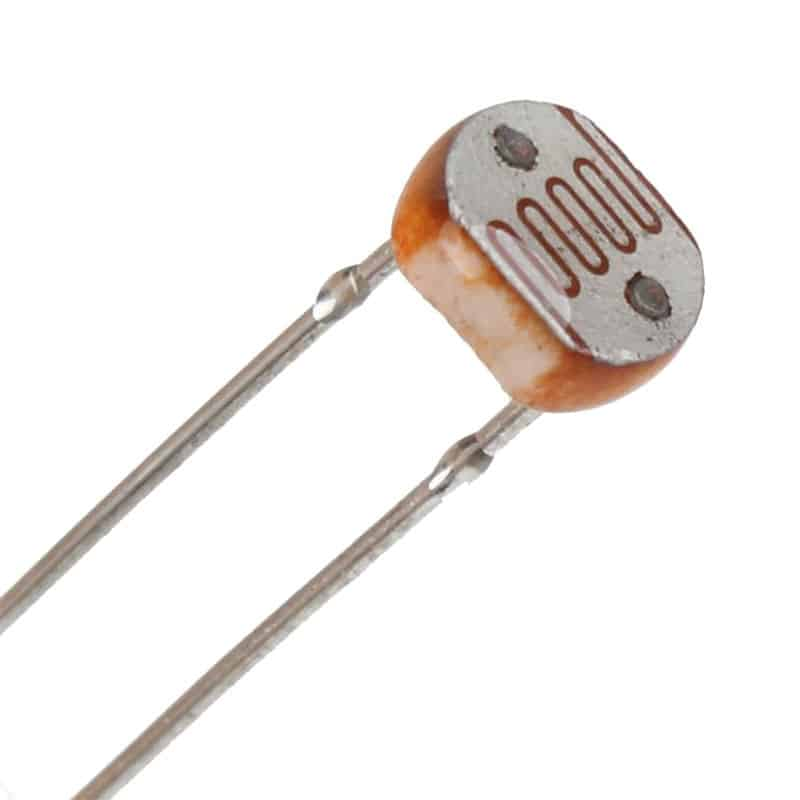
\includegraphics[scale=0.15]{./Figures/ldr.jpg}
		\caption{Fotoresistencia GL5528\protect\footnotemark.}
		\label{fig:cuadradoAzul}
	\end{figure}
	
	\footnotetext{Imagen tomada de: \url{https://www.devobox.com/en/photosensors/38-photoresistor-ldr07.html}}
	
	\item Fototransistor: es un transistor sensible a la luz, normalmente a los infrarrojos. La cantidad de luz incidente es proporcional a la corriente de base generada. Generalmente tiene el factor de forma de un LED \citep{BOOK:2}. Un fototransistor de uso común se observa en la figura 2.3.
\end{itemize}

	\begin{figure}[h]
		\centering
		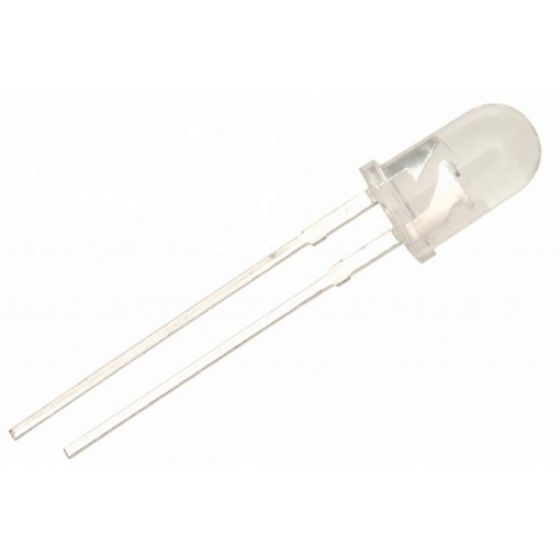
\includegraphics[scale=0.3]{./Figures/phototransistor.jpg}
		\caption{Fototransistor IR333C\protect\footnotemark.}
		\label{fig:cuadradoAzul}
	\end{figure}

	\footnotetext{Imagen tomada de: \url{https://www.steren.com.gt/fototransistor-de-5-mm-transparente.html}}

\subsection{Microcontrolador}

\subsection{Transceptor Wi-Fi}

Wi-Fi es un tecnología de red inalámbrica, que permite a dispositivos como computadoras y teléfonos celulares conectarse entre sí para formar una red, o conectarse a un enrutador por el que se disponga de conexión a Internet. Está basado en la familia de estándares IEEE 802.11, que definen los protocolos que permiten la comunicación entre dispositivos compatibles con Wi-Fi \citep{WEBSITE:11}.Según la versión de Wi-Fi, puede funcionar en las bandas de 2.4 GHz o 5 GHz\citep{WEBSITE:11}.

En la tabla 2.1 muestran las características técnicas de las distintas versiones del estándar IEEE 802.11.

\begin{table}[h]
	\centering
	\caption[IEEE 802.11]{Tabla comparativa de características del estándar IEEE 802.11\protect\footnotemark}
	\begin{tabular}{l c c c}    
		\toprule
		\textbf{Protocolo 802.11} & \textbf{Frecuencia} & \textbf{Ancho de banda} & \textbf{Velocidad de datos (Mb/s)} \\
		\midrule
		a & 5 GHz 			& 20 MHz 		  & 5, 9, 12, 18, 24, 36, 48, 54 \\		
		b & 2.4 GHz			& 20 MHz 		  & 1, 2, 5.5, 11 \\
		g & 2.4 GHz			& 20 MHz          & 6, 9, 12, 18, 24, 36, 48, 54 \\
		n & 2.4 GHz y 5 GHz & 20 MHz y 40 MHz & 7.2, 28.9, 43.3, 57.8, 65, 72.2 \\
		\bottomrule
		\hline
	\end{tabular}
	\label{tab:peces}
\end{table}

\footnotetext{Datos obtenidos de: \url{https://microchipdeveloper.com/wifi:a-b-g-n-explained}}

Dentro del modelo OSI\footnote{Modelo OSI. Es un modelo de referencia para los protocolos de red, creado por la Organización Internacional de Normalización.}, Wi-Fi se encuentra en la capa física y de enlace de datos. En la figura 2.x se ve el modelo OSI.
\begin{figure}[h]
	\centering
	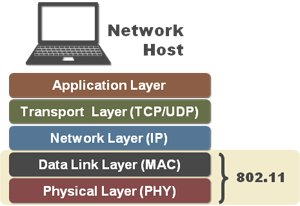
\includegraphics[scale=0.7]{./Figures/osi_model.jpg}
	\caption{Ubicación de Wi-Fi en el modelo OSI\protect\footnotemark.}
	\label{fig:cuadradoAzul}
\end{figure}

\footnotetext{Imagen tomada de: \url{https://microchipdeveloper.com/wifi:80211-osi}}

Una red Wi-Fi tiene una arquitectura en estrella como se muestra en la figura 2.x. 

\begin{figure}[h]
	\centering
	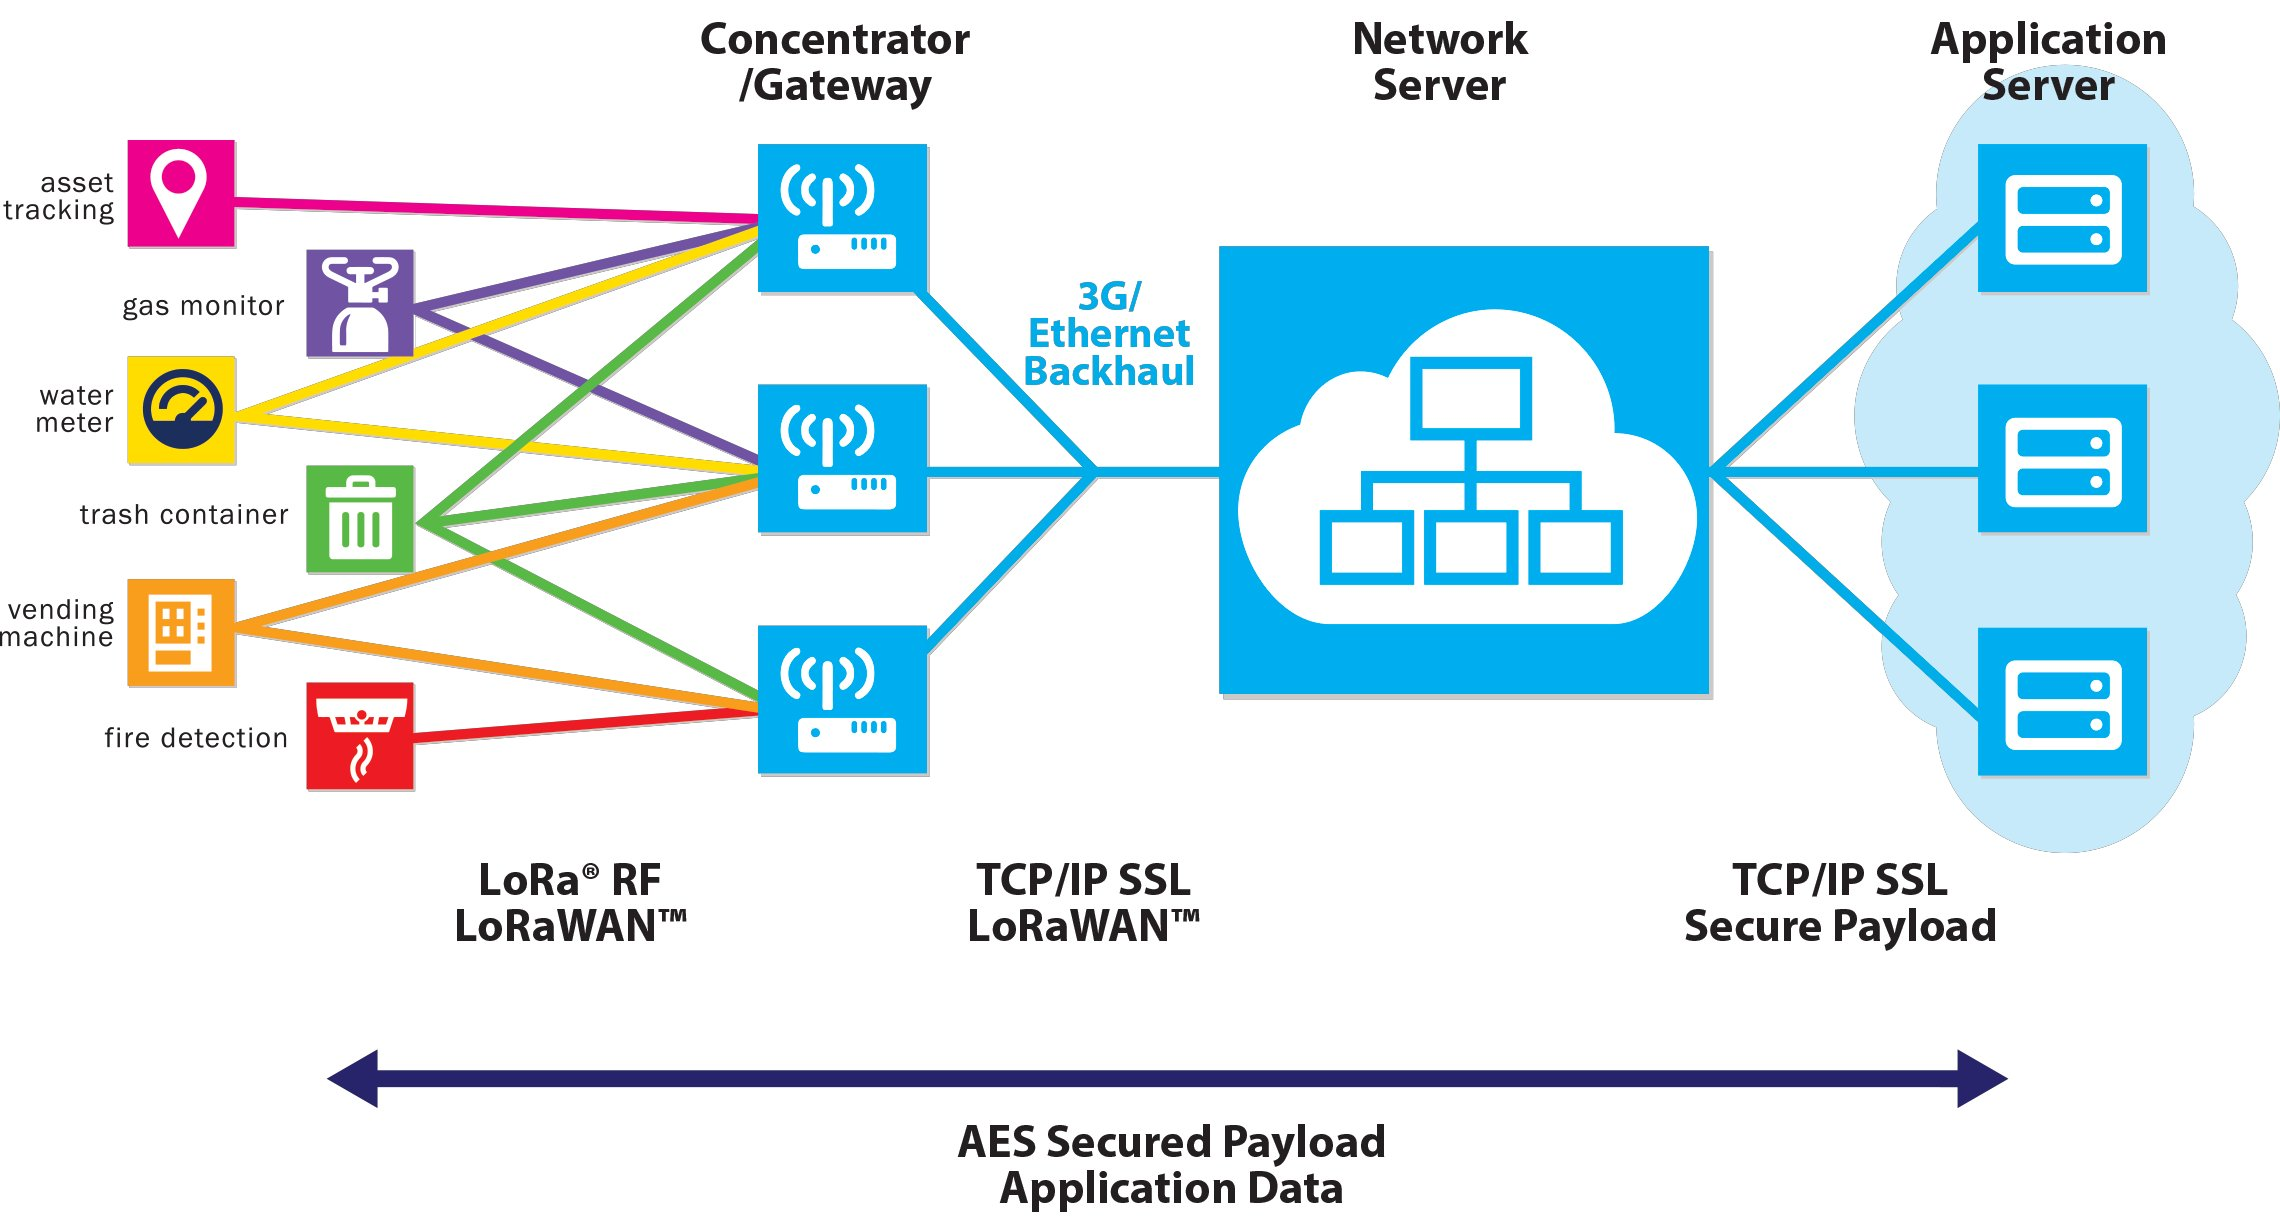
\includegraphics[scale=0.17]{./Figures/lorawan_architecture.jpg}
	\caption{Arquitectura LoraWAN\protect\footnotemark.}
	\label{fig:cuadradoAzul}
\end{figure}

\footnotetext{Imagen tomada de: \url{https://www.aprendiendoarduino.com/2018/03/05/redes-lpwan/}}

Los elementos principales de una red Wi-Fi son:
\begin{itemize}
	\item Estaciones: son dispositivos electrónicos que se conectan entre sí a través de enrutadores inalámbricos. Son más conocidos como hosts y pueden ser computadoras, tabletas, teléfonos celulares o sistemas embebidos.
	\item Puntos de acceso: también conocidos como \textit{Access Points}, son los elementos de la red que enrutan la información proveniente de las estaciones dentro de la red local o hacia otras redes.
\end{itemize}

Dentro de lo referido al desarrollo de sistemas embebidos, comercialmente pueden encontrarse módulos Wi-Fi como el de la figura 2.x.

\begin{figure}[h]
	\centering
	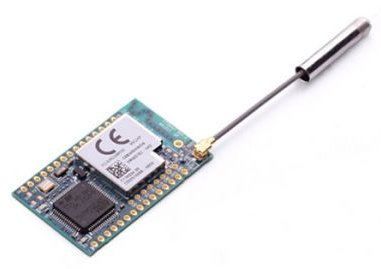
\includegraphics[scale=0.65]{./Figures/wifi_module.jpg}
	\caption{Módulo Wi-Fi basado en el circuito integrado EMW3162\protect\footnotemark.}
	\label{fig:cuadradoAzul}
\end{figure}

\footnotetext{Imagen tomada de: \url{https://www.seeedstudio.com/EMW3162-WiFi-Module-External-IPEX-antenn-p-2235.html}}

\subsection{Transceptor LoRa}

LoRa(\textit{Long Range}, largo alcance), es una técnica de modulación de espectro extendido derivada de la tecnología CSS (\textit{Chirp Spread Spectrum}, espectro extendido de tipo chirp)\citep{WEBSITE:9}. Fue desarrollado por la firma Semtech y es utilizada principalmente en dispositivos orientados a IoT(\textit{Internet of Things}, Internet de las cosas) y dispositivos alimentados por baterías. Opera en las bandas de 433 Mhz, 868 Mhz y 915 MHz, según el país.

Las comunicaciones entre dispositivos LoRa, son del tipo punto a punto, ya que la tecnología es de capa física. Para formar redes LoRa, es necesaria una capa MAC (\textit{Media Access Control}, control de acceso al medio), la cual es llamada LoRaWAN (\textit{Long Range Wide Area Network}, red de área amplia LoRa).

LoRaWAN, es una especificación de redes LPWAN (\textit{Low Power Wide Area Network}, red de área amplia de baja potencia) y LoRa Alliance es la encargada de su estandarización. Está diseñada para conectar dispositivos de bajo consumo energético a Internet a través de redes regionales, nacionales o globales. Además proporciona comunicación bidireccional, seguridad, movilidad y servicios de localización\citep{WEBSITE:10}.

En la figura 2.x se puede observar el modelo de capas de una red de dispositivos LoRa, donde el protocolo LoRa define la capa física (PHY) y LoRaWAN la capa de acceso al medio (MAC).

\begin{figure}[h]
	\centering
	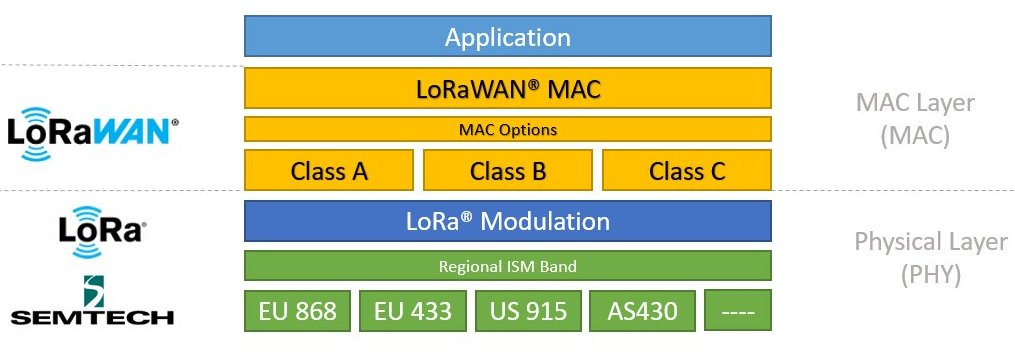
\includegraphics[scale=0.38]{./Figures/lorawan.jpg}
	\caption{\textit{Stack} LoraWAN\protect\footnotemark.}
	\label{fig:cuadradoAzul}
\end{figure}

\footnotetext{Imagen tomada de: \url{https://lora-developers.semtech.com/library/tech-papers-and-guides/lora-and-lorawan/}}

La arquitectura de una red LoRaWAN es de tipo estrella, como se muestra en la figura 2.x.

\begin{figure}[h]
	\centering
	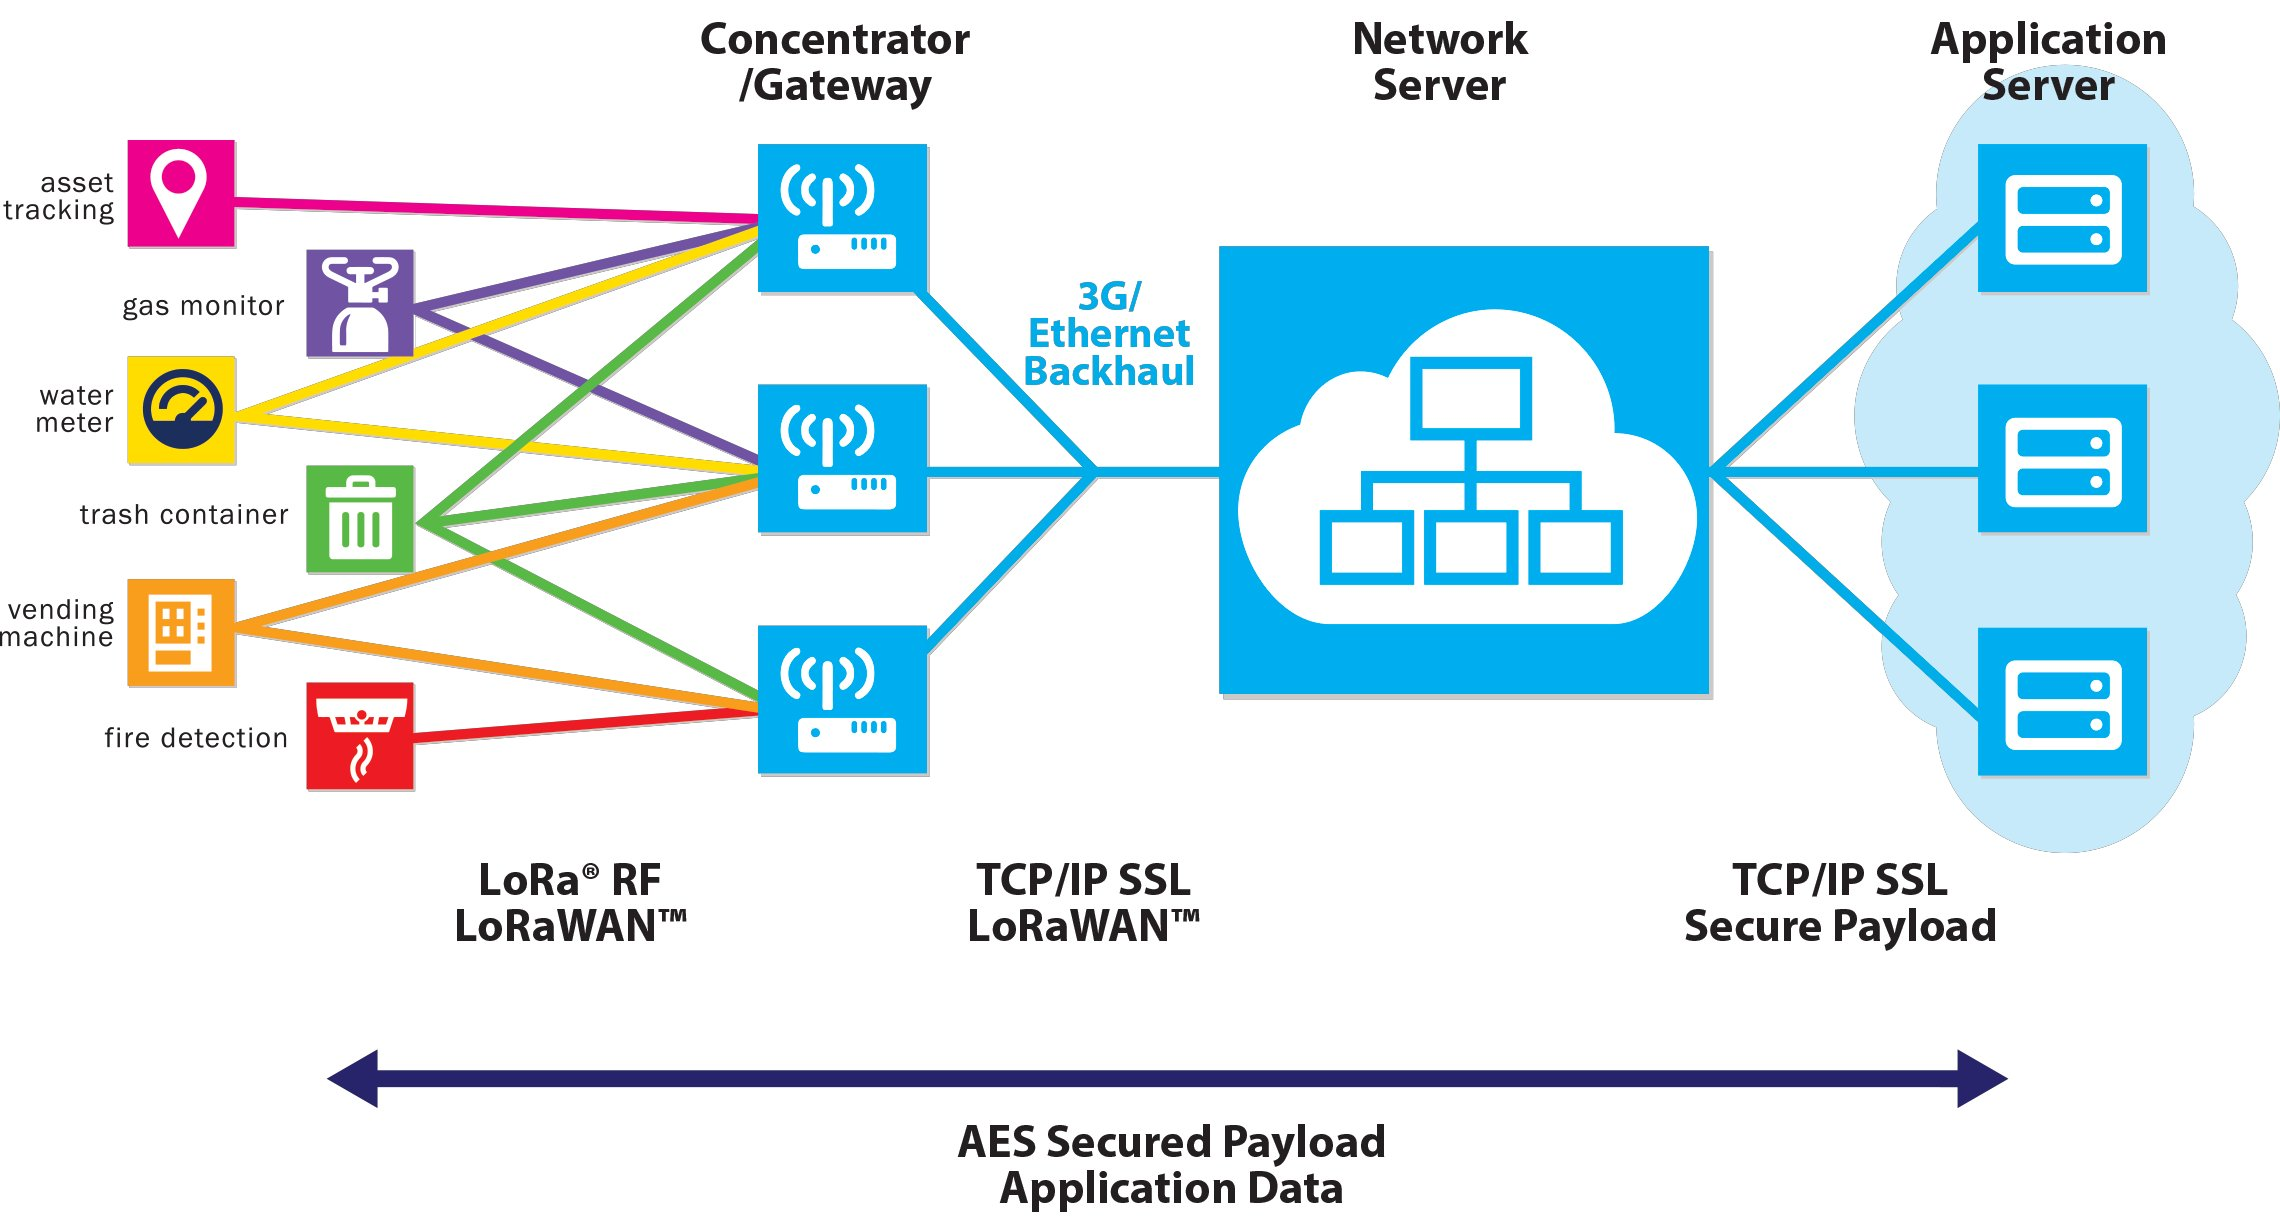
\includegraphics[scale=0.17]{./Figures/lorawan_architecture.jpg}
	\caption{Arquitectura LoraWAN\protect\footnotemark.}
	\label{fig:cuadradoAzul}
\end{figure}

\footnotetext{Imagen tomada de: \url{https://www.aprendiendoarduino.com/2018/03/05/redes-lpwan/}}

De la figura anterior, se distinguen los siguientes elementos:

\begin{itemize}
	\item Nodos: son los dispositivos que utilizan la tecnología LoRa como método de transmisión de datos. Son utilizados para obtener datos de sensores o para interactuar con actuadores. Generalmente son dispositivos de bajo consumo energético y alimentados por baterías.
	\item Concentradores: también conocidos como \textit{gateways}, son los encargados de recibir la información de los nodos y reenviarla a un servidor de red. Estos dispositivos tienen acceso a Internet mediante redes celulares, Wi-Fi o \textit{ethernet}.
	\item Servidores de red: son los responsables del enrutamiento de los mensajes a la aplicación adecuada, seleccionar el mejor gateway para el mensaje de enlace descendente, eliminar mensajes duplicados y descifrar los mensajes que vienen cifrados desde los nodos.
	\item Servidores de aplicación: es donde se realizan los procesos útiles sobre los datos obtenidos de los nodos. Típicamente se ejecutan en una nube privada o pública.
\end{itemize}

En el desarrollo de nodos para redes LoRaWAN, se utilizan módulos de desarrollo que llevan embebido un circuito integrado con tecnología LoRa, como el de la figura 2.x.

\begin{figure}[h]
	\centering
	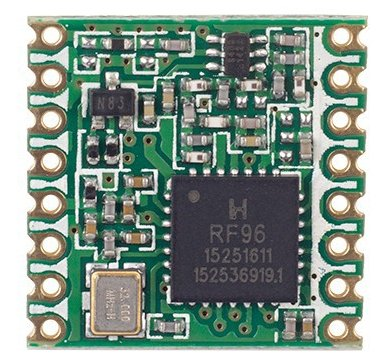
\includegraphics[scale=0.32]{./Figures/lora_module.jpg}
	\caption{Módulo LoRa basado en el circuito integrado RF96\protect\footnotemark.}
	\label{fig:cuadradoAzul}
\end{figure}

\footnotetext{Imagen tomada de: \url{https://www.antratek.com/rfm95-lora-module}}

\subsection{Reloj en tiempo real}

Más conocido como RTC (\textit{Real-Time Clock}, reloj en tiempo real), es un circuito integrado que tiene la capacidad de llevar con precisión la hora y fecha. Para contar con exactitud los segundos, utiliza un oscilador de cristal de cuarzo de 32.768 kHz, que puede o no estar embebido en el encapsulado del RTC.

La principal aplicación de un RTC es brindar a un sistema electrónico la hora y fecha exactas,  también puede ofrecer otras funciones como alarmas, salidas de reloj de 1 Hz o medición de temperatura.

Algunos RTCs tienen una fuente de poder alternativa basada en baterías, que mantiene funcionando la parte del circuito que lleva la cuenta de la hora y fecha. Esta fuente de tensión normalmente son baterías de litio o supercapacitores\footnote{Supercapacitor. Es un capacitor que tiene valores de capacitancia muy altos, pero valores de voltaje muy bajos.}. Comercialmente un RTC puede adquirirse como parte de un módulo, como el que se ve en la figura 2.4, que tiene instalada la fuente de alimentación alternativa y brinda mayor facilidad para acceder a los pines del circuito integrado.

\begin{figure}[h]
	\centering
	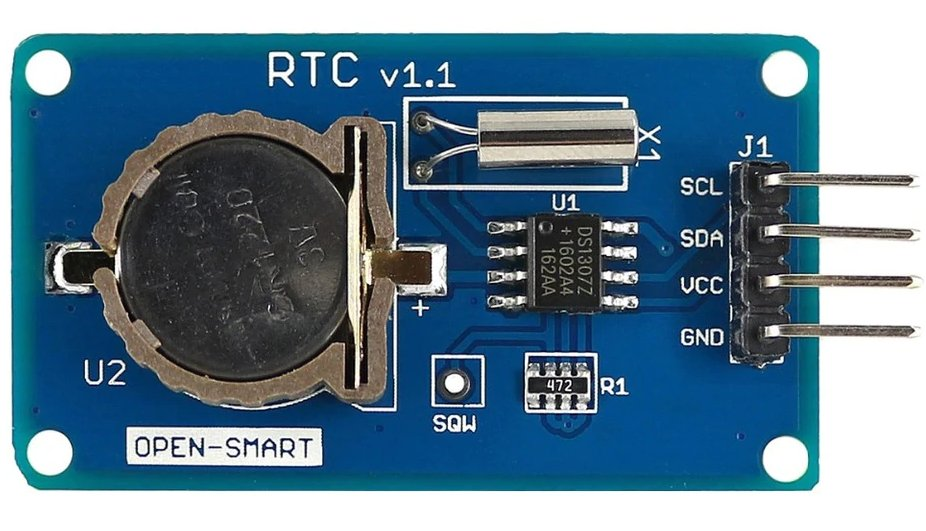
\includegraphics[scale=0.2]{./Figures/rtc.jpg}
	\caption{Módulo RTC basado en el circuito integrado DS1307.}
	\label{fig:cuadradoAzul}
\end{figure}

\subsection{Memoria no volátil}

Es un tipo de memoria de lectura y escritura, en la que los datos que tiene almacenados se mantienen intactos cuando la fuente de alimentación deja de funcionar, es decir, que no necesita energía para mantener guardada la información grabada en ella \citep{BOOK:3}.

En sistemas embebidos, existen principalmente dos tipos de memorias no volátiles:

\begin{itemize}
	\item EEPROM (\textit{Electrically Erasable Programmable Read-Only Memory}, ROM borrable y programable eléctricamente): es un tipo de memoria ROM que puede ser programada y borrada mediante métodos eléctricos. Aunque puede ser leída un número ilimitado de veces, las operaciones de escritura o borrado de datos solo se pueden realizar entre cien mil y un millón de veces. Este tipo de memorias pueden encontrarse como circuitos integrados que generalmente disponen de comunicación I2C o SPI. En la figura 2.5 se aprecia un módulo EEPROM, comercialmente esta es la forma más habitual de encontrarlo.
	\begin{figure}[h]
		\centering
		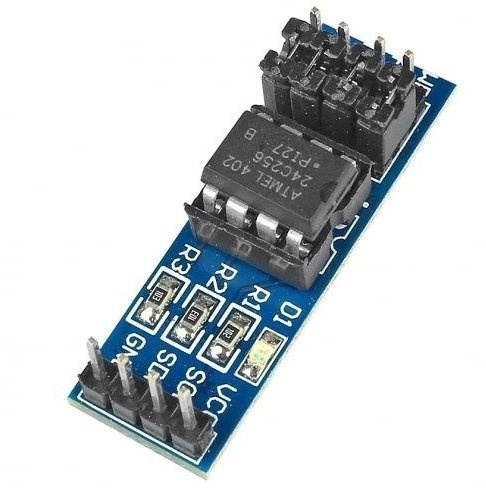
\includegraphics[scale=0.35]{./Figures/eeprom.jpg}
		\caption{Módulo EEPROM basado en el circuito integrado 24C256.}
		\label{fig:cuadradoAzul}
	\end{figure}
	\item Flash: está basada en las memorias EEPROM y permite la lectura y escritura de múltiples posiciones de memoria de manera simultánea, gracias a ello su velocidad de funcionamiento es superior a la de su antecesor. El número de operaciones de escritura o borrado es de diez mil a un millón. Es empleada principalmente en la fabricación de memorias USB y unidades de estado sólido. Asimismo, los microcontroladores actuales tienen integrada una unidad de memoria flash para el almacenamiento de instrucciones y datos. Para la realización de pruebas y prototipos, existen comercialmente módulos de memoria flash con comunicación SPI, como el de la figura 3.6.
	\begin{figure}[h]
		\centering
		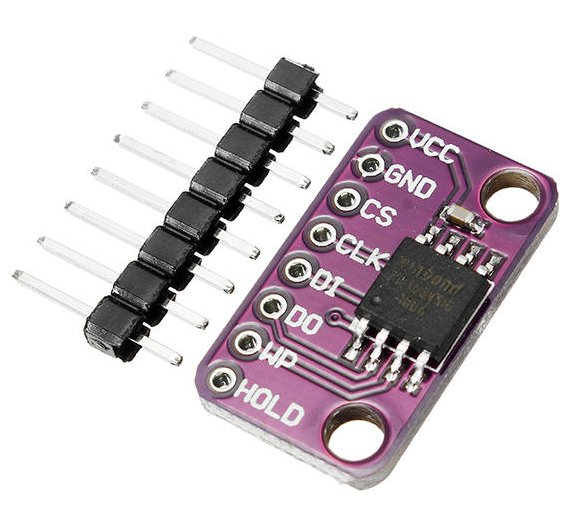
\includegraphics[scale=0.35]{./Figures/flash.jpg}
		\caption{Módulo flash basado en el circuito integrado W25Q16BVSIG.}
		\label{fig:cuadradoAzul}
	\end{figure}
	
\end{itemize}

%----------------------------------------------------------------------------------------

\section{Planificación}

Como se explicó en la subsección 2.2, el dispositivo esta compuesto por diferentes bloques funcionales, que tienen tanto componentes de firmware como de hardware. 
dsadasdasd
asdasdsadas
dasdsa
dsad
sad

%---------------------------------------------------------------------------------------- 
\chapter{Diseño e implementación} % Main chapter title

\label{Chapter3} % Change X to a consecutive number; for referencing this chapter elsewhere, use \ref{ChapterX}

\definecolor{mygreen}{rgb}{0,0.6,0}
\definecolor{mygray}{rgb}{0.5,0.5,0.5}
\definecolor{mymauve}{rgb}{0.58,0,0.82}

%%%%%%%%%%%%%%%%%%%%%%%%%%%%%%%%%%%%%%%%%%%%%%%%%%%%%%%%%%%%%%%%%%%%%%%%%%%%%
% parámetros para configurar el formato del código en los entornos lstlisting
%%%%%%%%%%%%%%%%%%%%%%%%%%%%%%%%%%%%%%%%%%%%%%%%%%%%%%%%%%%%%%%%%%%%%%%%%%%%%
\lstset{ %
  backgroundcolor=\color{white},   % choose the background color; you must add \usepackage{color} or \usepackage{xcolor}
  basicstyle=\footnotesize,        % the size of the fonts that are used for the code
  breakatwhitespace=false,         % sets if automatic breaks should only happen at whitespace
  breaklines=true,                 % sets automatic line breaking
  captionpos=b,                    % sets the caption-position to bottom
  commentstyle=\color{mygreen},    % comment style
  deletekeywords={...},            % if you want to delete keywords from the given language
  %escapeinside={\%*}{*)},          % if you want to add LaTeX within your code
  %extendedchars=true,              % lets you use non-ASCII characters; for 8-bits encodings only, does not work with UTF-8
  %frame=single,	                % adds a frame around the code
  keepspaces=true,                 % keeps spaces in text, useful for keeping indentation of code (possibly needs columns=flexible)
  keywordstyle=\color{blue},       % keyword style
  language=[ANSI]C,                % the language of the code
  %otherkeywords={*,...},           % if you want to add more keywords to the set
  numbers=left,                    % where to put the line-numbers; possible values are (none, left, right)
  numbersep=5pt,                   % how far the line-numbers are from the code
  numberstyle=\tiny\color{mygray}, % the style that is used for the line-numbers
  rulecolor=\color{black},         % if not set, the frame-color may be changed on line-breaks within not-black text (e.g. comments (green here))
  showspaces=false,                % show spaces everywhere adding particular underscores; it overrides 'showstringspaces'
  showstringspaces=false,          % underline spaces within strings only
  showtabs=false,                  % show tabs within strings adding particular underscores
  stepnumber=1,                    % the step between two line-numbers. If it's 1, each line will be numbered
  stringstyle=\color{mymauve},     % string literal style
  tabsize=2,	                   % sets default tabsize to 2 spaces
  title=\lstname,                  % show the filename of files included with \lstinputlisting; also try caption instead of title
  morecomment=[s]{/*}{*/}
}


%----------------------------------------------------------------------------------------

En este capítulo se explica el proceso que se siguió para desarrollar e implementar el prototipo de pruebas, el firmware, la interfaz web y el prototipo comercial.`

%----------------------------------------------------------------------------------------

\section{Prototipo de pruebas}

El prototipo de pruebas fue desarrollado con la finalidad de probar todas las funciones de firmware que componen el trabajo, para brindar una primera aproximación al prototipo comercial del dispositivo.

Como se vio en el diagrama de la figura \ref{fig:diagramBlocks}, el dispositivo está compuesto por los siguientes bloques funcionales: microcontrolador, transceptor Wi-Fi, transceptor LoRa, memoria no volátil, reloj en tiempo real y conversor óptico-eléctrico.

La construcción del prototipo de pruebas se realizó en una \textit{breadboard}, que pemitió realizar cambios en las conexiones de los componentes de una manera sencilla cuando estos se requerían. Se eligieron componentes de hardware acordes con los bloques que constituyen el dispositivo, en su mayor parte módulos de desarrollo con circuitos integrados embebidos que disponen de conectores apropiados para una breadboard. En la figura \ref{fig:blocksTest} se muestra el diagrama en bloques general con los componentes del prototipo de pruebas.

\begin{figure}[h]
	\centering
	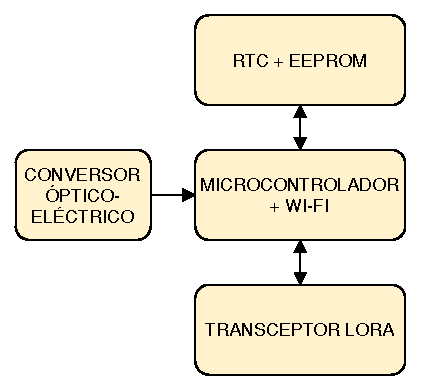
\includegraphics[scale=1]{./Figures/test_blocks.pdf}
	\caption{Diagrama en bloques del prototipo de pruebas.}
	\label{fig:blocksTest}
\end{figure}

Para garantizar un tiempo corto en la obtención de los componentes del prototipo de pruebas, el criterio predominante para la elección de los componentesfue la disponibilidad en el mercado local. Además, la elección de proveedores locales aseguró la restitución eficaz de los componentes que se malograron durante el desarrollo.

\subsection{Microcontrolador + Wi-Fi}

Este bloque fusiona los bloques microcontrolador y transceptor Wi-Fi. El desarrollo de dispositivos con conexión Wi-Fi ha tenido un gran crecimiento en los últimos años \citep{WEBSITE:19}, por lo que existen algunos fabricantes de circuitos integrados que ofrecen soluciones que integran microcontroladores y transceptores Wi-Fi en un solo encapsulado.

El componente elegido para este bloque es la tarjeta de desarrollo NodeMCU de la firma Amica, basado en el módulo ESP-12F de la firma Ai-Thinker. Las características más atractivas de esta tarjeta en lo referente al desarrollo son: alimentación y programación a través de un puerto micro USB, factor de forma adecuado para ser montado sobre un breadboard e incorporación de LEDs y pulsadores en la misma tarjeta. En la figura 3.2 se muestra la NodeMCU.

\begin{figure}[h]
	\centering
	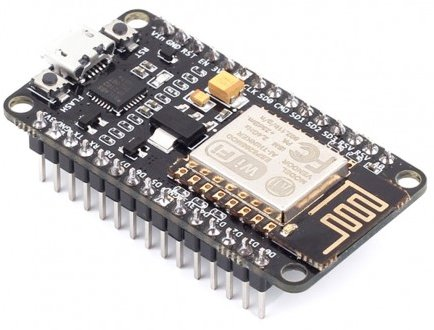
\includegraphics[scale=0.5]{./Figures/nodemcu.jpg}
	\caption{Tarjeta de desarrollo NodeMCU de la firma Amica\protect\footnotemark.}
		\label{fig:nodemcu}
	\end{figure}

	\footnotetext{Imagen tomada de: \url{https://www.amazon.com/-/es/KeeYees-Internet-Development-Wireless-Compatible/dp/B07PR9T5R5}}

El módulo ESP-12F monta sobre sí un SoC (\textit{System on a Chip}, sistema en un chip) de la firma Espressif Systems, el ESP8266, que funciona como microcontrolador y transceptor Wi.Fi. Otros componentes instalados sobre este módulo son condensadores, resistencias, oscilador, memoria flash y una antena impresa; todos ellos necesarios para que el ESP8266 pueda desempeñar correctamente sus funciones.

El ESP8266 es un chip de bajo costo que incorpora un microcontrolador y un transceptor Wi-Fi, además de contar con un \textit{stack} TCP/IP. Sus características técnicas más relevantes son:
\begin{itemize}
	\item Procesador Tensilica LX106 de arquitectura RISC(footnote) de 32 bits a una frecuencia de 80 MHz.
	\item RAM de 64 KB para instrucciones y 96 KB para datos.
	\item ROM externa, puede soportar hasta 16 MB de memoria flash con conexión QSPI(footnote).
	\item IEEE 802.11 b/g/n.
	\item Periféricos GPIO, SPI, I\textsuperscript{2}C, UART y ADC.
\end{itemize}

\subsection{Transceptor LoRa}

Para la elección del componente de este bloque hubieron varias consideraciones, la más importante fue la frecuencia de transmisión y recepción. LoRa trabaja en las frecuencias de 433 MHz, 868 MHz y 915 MHz; de acuerdo al país donde se implementa. Esto en Bolivia está normado por la Autoridad de Regulación y Fiscalización de Telecomunicaciones y Transportes, ATT, a través del documento de plan de frecuencias \citep{WEBSITE:17}. En dicho documento se determina la frecuencia de 915 MHZ como la banda destinada para este tipo de aplicaciones.

En el mercado local no se pudieron encontrar módulos LoRa que funcionen a la frecuencia de 915 MHz. Se adquirieron los módulos disponibles, que trabajan en la frecuencia de 433 MHz, lo que según \citep{WEBSITE:17} está destinado a radioaficionados. El módulo utilizado para el prototipo de pruebas fue el PM1280, que está basado el circuito integrado SX1278. En la figura \ref{fig:loraModule} se observa una fotografía del módulo PM1280.

\begin{figure}[h]
	\centering
	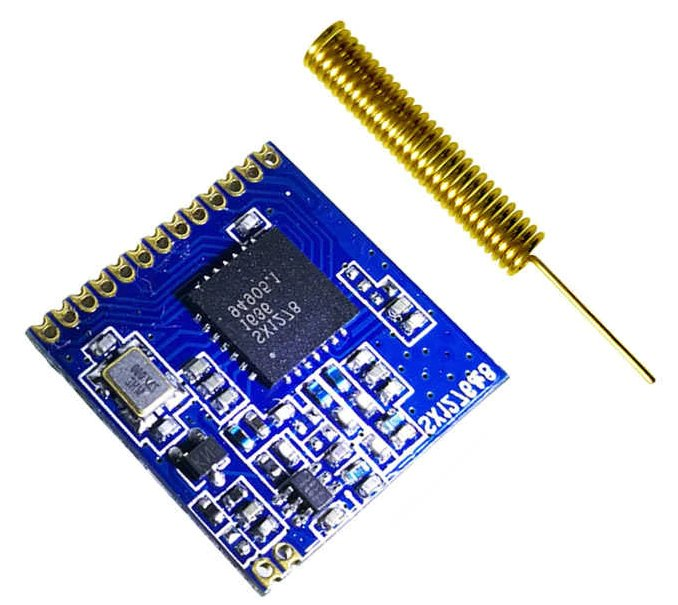
\includegraphics[scale=0.3]{./Figures/pm1280.jpg}
	\caption{Módulo LoRa PM1280\protect\footnotemark.}
		\label{fig:loraModule}
\end{figure}

\footnotetext{Imagen tomada de: \url{https://www.todomicro.com.ar/arduino/910-modulorf-lora-sx1278-chip-pm1280-con-antena.html}}

El circuito integrado SX1278 es un transceptor LoRa de la firma Semtech que provee comunicación de espectro ensanchado de largo alcance y alta inmunidad a las interferencias. Su principales características son:

\begin{itemize}
	\item Potencia de transmisión de 100mW.
	\item Alta eficiencia del amplificador de potencia.
	\item Frecuencia de operación: 137 MHZ a 525 MHZ.
	\item Velocidad de bit programable hasta 300 Kbps.
	\item Bajo consumo de corriente, 9,9 mA en modo de recepción y 200 nA en la retención de datos en sus registros.
	\item Soporta paquetes de hasta 256 bytes.
	\item Sensor de temperatura e indicador de batería incorporado.
\end{itemize}


\subsection{RTC + EEPROM}

Los bloques memoria no volátil y reloj en tiempo real fueron fusionados en un único bloque, ya que comercialmente existen módulos que cumplen ambas funciones. Estos módulos tienen embebidos circuitos integrados de memoria y RTC, además de otros componentes como resistencias, condensadores, osciladores, zócalos para baterías y conectores apropiados para un breadboard. Estos módulos en su gran mayoría poseen una EEPROM como medio de almacenamiento de datos, esta tecnología es preferible sobre las memorias flash en aplicaciones de adquisición de datos, ya que proporciona un número mayor de ciclos de escritura y borrado.

La mayor parte de los módulos que existen en el mercado local cumplen cabalmente con las funciones que requiere este bloque, pero debido a la cantidad de pines utilizables de la NodeMCU se tuvo preferencia por los módulos que tenían integrados chips con interfaz I\textsuperscript{2}C. Asimismo, al haber muchos módulos que cumplían el requisito de la interfaz, se buscó uno que tuviera un RTC con la capacidad de generar alarmas en función de la hora. En la figura 3.2 se observa el módulo de RTC + EEPROM elegido.

\begin{figure}[h]
	\centering
	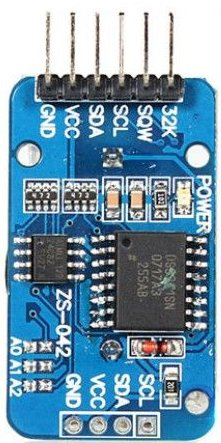
\includegraphics[scale=0.4]{./Figures/rtc_eeprom.jpg}
	\caption{Módulo RTC + EEPROM\protect\footnotemark.}
		\label{fig:cuadradoAzul}
	\end{figure}

	\footnotetext{Imagen tomada de: \url{https://electropeak.com/extremely-accurate-rtc-module}}

Los circuitos integrados que componen el módulo son el DS3231 y el AT24C32, un RTC y una EEPROM, respectivamente. El DS3231 es un RTC de alta precisión de la firma Maxim Integrated, que cuenta con una interfaz I\textsuperscript{2}C para conectarse con otros dispositivos, también tiene la capacidad de generar alarmas y medir la temperatura. El AT24C32 es una EEPROM de la firma Microchip, con interfaz I\textsuperscript{2}C y 32 KB de capacidad de almacenamiento.

\subsection{Conversor óptico-eléctrico}

Para este bloque, el componente elegido es un módulo detector de luz, compuesto por un fototransistor PT333-3C de la firma Everlight y un comparador de voltaje LM393 de la firma Texas Instruments. El módulo genera como salida un pulso eléctrico acotado al nivel de tensión con el que se alimenta. Cuando la cantidad de luz incidente en el fototransistor provoca un nivel de tensión igual o mayor al nivel de tensión del potenciómetro que viene incluido. En la figura \ref{fig:coeModule} se puede observar el módulo.

\begin{figure}[h]
	\centering
	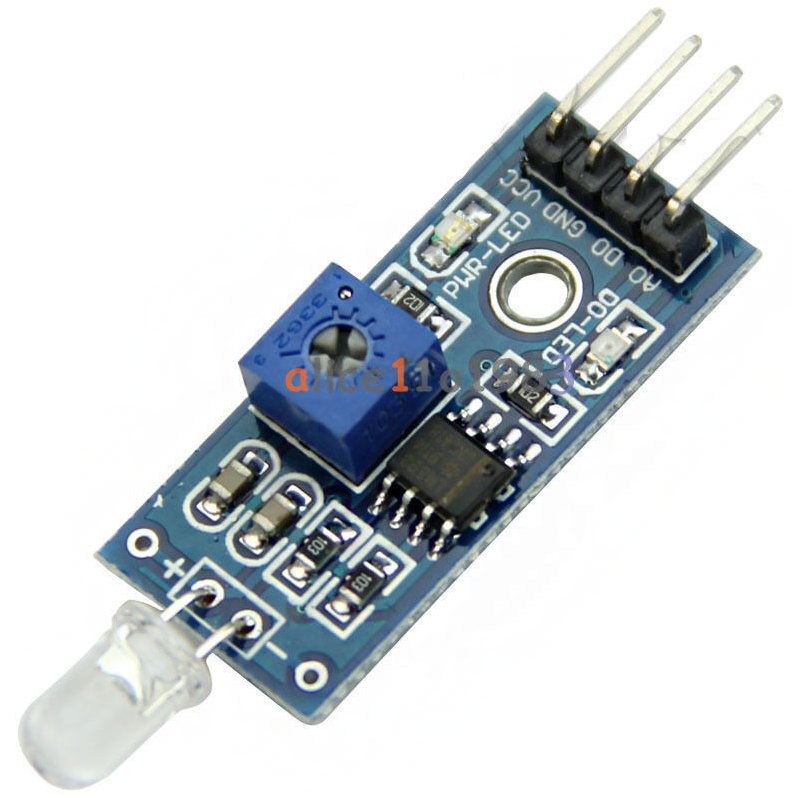
\includegraphics[scale=0.2]{./Figures/coe.jpg}
	\caption{Módulo detector de luz\protect\footnotemark.}
		\label{fig:coeModule}
\end{figure}

	\footnotetext{Imagen tomada de: \url{https://www.roboter-bausatz.de/en/diy-electronics/extension-modules/sensors/optics-light/149/light-sensor-module}}

%----------------------------------------------------------------------------------------

\section{Diseño de firmware}

El desarrollo del firmware fue la actividad que requirió más esfuerzo en el trabajo, debido a que los objetivos principales del autor fueron lograr modularización y reutilización del código escrito. Para lograr dichos objetivos, el firmware fue estructurado en capas y se utilizó control de versiones para documentarlo. De esta manera, se logró un desarrollo de carácter más profesional que podría ser reutilizado en futuros proyectos que requieran funciones similares.

Antes de realizar la descomposición del firmware en capas, fue necesario elegir las herramientas de desarrollo implicadas, que fueron imprescindibles al momento de escribir el código fuente del dispositivo. Estas herramientas fueron un SDK (\textit{Software Deveplopment Kit}, kit de desarrollo de software) que proporcionó una API (\textit{Application Programming Interface}, interfaz de programación de aplicaciones) para facilitar el desarrollo de código fuente para el ESP8266 y un IDE (\textit{Integrated Development Enviroment}, Entorno de Desarrollo Integrado) que proporcionó un entorno con herramientas que agilizaron la escritura de código con el SDK elegido. Estos fueron:

\begin{itemize}
	\item ESP8266\_RTOS\_SDK: este SDK fue desarrollado por la firma Espressif Systems para la programación del SoC ESP8266 y facilita un conjunto de funciones para la creación de código fuente. Está basado en el RTOS (\textit{Real-Time Operating System}, sistema operativo en tiempo real) de uso gratuito FreeRTOS \citep{WEBSITE:18}, que fue utilizado en las materias sobre sistemas operativos en tiempo real de la Carrera de Especialización y brindó funciones que ayudaron a lograr determinismo en la ejecución de las tareas del dispositivo. Asimismo, contiene bastante documentación y ejemplos sobre como utilizar las funciones del ESP8266.
	\item Eclipse: el aspecto más importante en la elección de este IDE, fue que en la documentación de instalación y uso del ESP8266\_RTOS\_SDK (ref), se indicaba el proceso de configuración de este Eclipse para compilar el código basado en este SDK. Otro aspecto de importancia fue la experiencia previa del autor con este IDE, el mismo fue utilizado en varias materias de la Carrera de Especialización.
\end{itemize}

Entonces, una vez definidas las herramientas utilizadas, fue posible dividir el firmware en capas para facilitar el desarrollo y reducir la complejidad del código escrito para el dispositivo. La división en capas del firmware puede observarse en el diagrama de la figura \ref{fig:firmwareLayers}, donde existen tres capas claramente diferenciadas: APP, DRIVERS y SDK.

\begin{figure}[h]
	\centering
	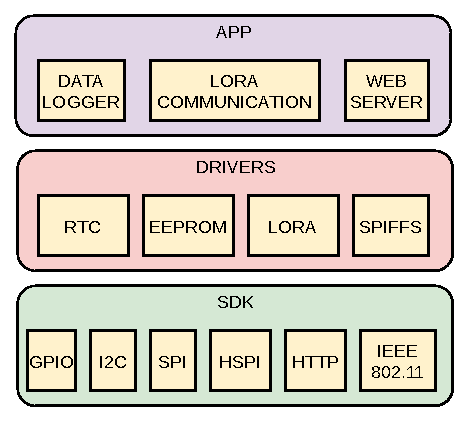
\includegraphics[scale=1]{./Figures/firmware_layers.pdf}
	\caption{Diagrama de capas del firmware.}
		\label{fig:firmwareLayers}
\end{figure}

SDK es la capa de menor nivel y está compuesta por la API del ESP8266\_RTOS\_SDK. Proporciona a las capas de niveles superiores la capacidad de interactuar con los periféricos y protocolos del ESP8266 a través de funciones en lenguaje C. De todos los periféricos y protocolos que dispone el ESP8266, los que fueron utilizados en el presente trabajo fueron:

\begin{itemize}
	\item GPIO: este periférico fue utilizado por la capa APP para gestionar los pines disponibles en el ESP8266, ya que algunos de ellos tienen funciones específicas y no pueden ser utilizados para propósitos generales. El SDK posee funciones para definir los pines como entradas o salidas, configuración de interrupciones por flanco positivo o negativo y resistencias de \textit{pull-up} internas.
	\item I\textsuperscript{2}C: se utilizó este periférico para que la capa DRIVERS mediante el protocolo I\textsuperscript{2}C interactúe con el RTC y la EEPROM. Al tener pocos pines disponibles en el ESP8266, este componente se hizo muy importante, ya que la comunicación con este protocolo solo requiere dos pines, uno para datos y otro para el reloj.
	\item SPI: la capa DRIVERS utiliza este periférico para comunicarse con el transceptor LoRa. El transceptor LoRa elegido, interacciona a través del protocolo SPI con el microcontrolador que lo maneja para intercambiar datos.
	\item HSPI: el ESP8266 no posee memoria ROM embebida en el SoC, por tanto, utiliza una memoria flash externa para almacenar las instrucciones del programa y los datos del usuario. Esta memoria flash se comunica con el ESP8266 mediante el protocolo HSPI. Este periférico se utilizó para que la capa DRIVERS configurare la flash como un sistema de archivos.
	\item HTTP: el SDK ofrece funciones para ejecutar este protocolo de transferencia de hipertexto. Fue de utilidad para proporcionar a la capa APP las funciones necesarias para implementar un servidor web capaz de responder a los métodos HTTP, GET y POST \citep{WEBSITE:20}.
	\item IEEE 802.11: el ESP8266 tiene embebida toda la electrónica necesaria para implementar los protocolos IEEE 802.11 en sus versiones b, g y n. La capa APP utilizó las funciones disponibles de este módulo para lograr que el dispositivo funcione como punto de acceso y/o estación.
\end{itemize}

La capa DRIVERS está compuesta por módulos que son bibliotecas de firmware, que le permiten al ESP8266 interactuar con los periféricos de hardware externos a los que está conectado. Se desarrollaron bibliotecas para los módulos EEPROM, RTC, LORA y SPIFFS; todos basados en las funciones proporcionadas por la capa SDK. Estas bibliotecas se encuentran en el repositorio del trabajo y constan de un archivo de código fuente y otro de cabecera, cada una.

La biblioteca para EEPROM se desarrolló con ayuda del \textit{datasheet}\footnote{\url{https://www.st.com/resource/en/datasheet/cd00001012.pdf}} del AT24C32, donde se indican todos los pormenores técnicos del funcionamiento de este circuito integrado. Además, se utilizaron las funciones de la capa SDK para gestionar correctamente la comunicación I\textsuperscript{2}C. Las funciones que proporciona esta biblioteca sirven para:

\begin{itemize}
	\item Leer de valores de 8, 16 y 32 bits de una dirección determinada de la EPROM.
	\item Escribir de valores de 8, 16 y 32 bits de una dirección determinada de la EPROM.
\end{itemize}

Para el módulo RTC se desarrolló una biblioteca que sirvió para configurar la hora, fecha y otras funciones incorporadas en el DS3231. La herramienta principal en el desarrollo de esta biblioteca fue el datasheet\footnote{\url{https://datasheets.maximintegrated.com/en/ds/DS3231.pdf}} de dicho circuito integrado, de este se obtuvo información sobre las direcciones de los registros que manejan sus funciones y la forma adecuada de configurarlos. Igual que para la biblioteca de EEPROM, las funciones de la capa SDK para el protocolo I\textsuperscript{2}C permitieron que se disponga de una manera para que el ESP8266 pueda intercambiar datos con el DS3231 con la menor cantidad de pines posible. Esta biblioteca permite:

\begin{itemize}
	\item Leer y configurar las horas, minutos y segundos.
	\item Leer y configurar el día, fecha, mes y año.
	\item Leer y configurar las dos alarmas disponibles.
	\item Leer y configurar las salidas digitales.
	
\end{itemize} 

El desarrollo de la biblioteca para el módulo LORA permitió manejar el circuito integrado SX1278, para establecer la comunicación de este elemento con el ESP8266 mediante el protcolo SPI. Esto permitió configurar sus parámetros para lograr la transmisión y recepción de datos con dispositivos de tecnología LoRa de manera exitosa. Está basada en la biblioteca Arduino LoRa de Sandeep Mistry \citep{WEBSITE:21} y en la información del datasheet\footnote{\url{https://cdn-shop.adafruit.com/product-files/3179/sx1276_77_78_79.pdf}} del SX1278. Asimismo, utiliza las funciones proporcionadas por la capa SDK para la comunicación por el protocolo SPI. Las funciones más importantes que proporciona son:

\begin{itemize}
	\item Configurar la frecuencia del módulo.
	\item Transmitir un \textit{buffer} de tamaño variable.
	\item Recibir datos en el buffer interno.
	\item Leer el valor del RSSI (\textit{Received Signal Strength Indication}, indicador de fuerza de la señal recibida) de los datos recibidos en el buffer interno.
	\item Establecer el modo de funcionamiento en bajo consumo.
	\item Configurar la potencia de transmisión.
	\item Configurar el SF (\textit{Spreading Factor}, factor de propagación).
	\item Configurar el ancho de banda.
	\item Habilitar/deshabilitar el CRC (\textit{Cyclic Redundancy Check}, verificación de redundancia cíclica).
\end{itemize}

Por último, se desarrollo una biblioteca para establecer un sistema de archivos muy reducido llamado SPIFFS (SPI \textit{Flash File System}, sistema de archivos flash SPI), que está albergado en la memoria flash externa utilizada para almacenar el programa del ESP8266. Esta biblioteca requirió menos esfuerzo en su desarrollo que las anteriores, debido a que la mayoría de las funciones necesarias para configurar el sistema de archivos son parte de ESP8266\_RTOS\_SDK y para le manejo de archivos se utilizaron las funciones estándar de C. Solo posee una función para inicializar el sistema de archivos, que configura la cantidad máxima de archivos y el tamaño.

El tamaño de este sistema de archivos es de 1 MB y fue configurado de acuerdo al tamaño total de la memoria flash, que en el módulo ESP-12F es de 4 MB. El restante se utilizó para el programa, datos de fábrica y datos de configuración de la interfaz física. El detalle de los archivos almacenados en SPIFFS puede observarse de la tabla \ref{tab:spiffsDetail}.

\begin{table}[h]
	\centering
	\caption[Contenido SPIFFS]{Tabla de detalle del contenido del sistema de archivos SPIFFS}
	\begin{tabular}{l c c}    
		\toprule
		\textbf{Nombre} & \textbf{Tamaño (KB)} & \textbf{Descripción} \\
		\midrule
		ajax-loadergif.gif & 6,2 & Imagen de carga de la interfaz web \\
		favicon.ico & 1,1 & Ícono de la interfaz web\\
		highchartsjs.gz	& 92 & Biblioteca JavaScript Highcharts comprimida \\
		highchartsmap.gz & 235,6 & Archivo de mapeo para highchartsjs.gz \\
		index.html & 7,3 & Documento HTML de la interfaz web \\
		jqueryjs.gz & 33,2 & Biblioteca JavaScript jQuery comprimida \\
		jquerymobilecss.gz & 25,1 & Hoja de estilos CSS de la bibliote jQuery Mobile \\
		jquerymobilejs.gz & 55,5 & Biblioteca JavaScript jQuery Mobile comprimida \\
		jquerymobilemap.gz & 88,8 & Archivo de mapeo para jquerymobilejs.gz \\
		config.txt & 0,6 & Archivo de configuración del dispositivo \\
		pulses.csv & 1 & Archivo con el registro histórico del consumo eléctrico \\
		
		\bottomrule
		\hline
	\end{tabular}
	\label{tab:spiffsDetail}
\end{table}

La mayoría de los archivos almacenados en SPIFFS son utilizados para generar la interfaz web, excepto config.txt y pulses.csv. El tamaño de memoria utilizado por todos los archivos es de 546,4 KB, que ocupa aproximadamente un 54\% del tamaño total del sistema de archivos. Hay que notar que los archivos de mayor tamaño fueron comprimidos antes de ser almacenados, ya que sin este proceso el tamaño total hubiera sido de 1,6 MB, que superaba aproximadamente en un 60 \% el tamaño del sistema de archivos.

La capa APP, está compuesta por los módulos que ejecutan las tareas del dispositivo. Se basa en las capas inferiores para interactuar con los periféricos del ESP8266 y con el hardware externo. Sus módulos son DATA LOGGER, LORA COMMUNICATION y WEB SERVER. Los archivos de estos módulos se encuentran en el repositorio del trabajo.

\subsection{DATA LOGGER}

Este módulo tiene la función de adquirir, procesar y almacenar la información de consumo eléctrico del medidor al que está instalado el dispositivo. Para este fin, se comunica con los módulos de las capas inferiores como se muestra en el diagrama de la figura \ref{fig:dataLayers}.

\begin{figure}[h]
	\centering
	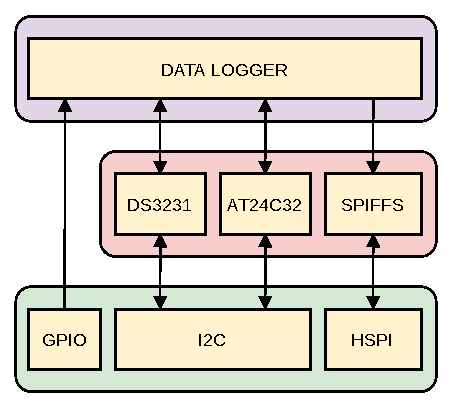
\includegraphics[scale=1]{./Figures/data_logger_diagram.pdf}
	\caption{Diagrama de capas para DATA LOGGER.}
		\label{fig:dataLayers}
\end{figure}

Utiliza el RTC y la EEPROM para mantener un registro histórico de la información adquirida por GPIO. Modifica el archivo pulses.csv almacenado en SPIFFS, para actualizar el registro histórico de consumo eléctrico cuando se registran nuevos datos, esto es utilizado posteriormente por WEB SERVER. Asimismo, en función de las alarmas generas por el RTC, se envían los datos de la EEPROM a LORA COMMUNICATION.

Dentro del sistema operativo utilizado existen dos tareas para este módulo. Una para registrar los pulsos del medidor eléctrico y otra para manejar las alarmas del RTC. Estas tareas utilizaron algunas herramientas proporcionadas por FreeRTOS para gestionar la forma en que se comunican los módulos. En la figura \ref{fig:dataRTOS} se observa un diagrama que muestra la manera en que se realiza la comunicación con ayuda de las herramientas de FreeRTOS.

\begin{figure}[h]
	\centering
	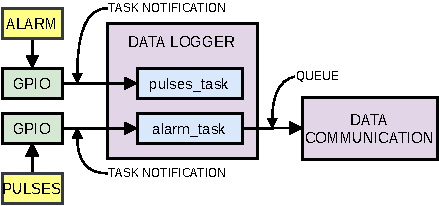
\includegraphics[scale=1]{./Figures/data_logger_com.pdf}
	\caption{Diagrama de conexión con las herramientas de FreeRTOS de DATA LOGGER.}
		\label{fig:dataRTOS}
\end{figure}

De la figura \ref{fig:dataRTOS}, ALARM representa las alarmas generadas por el RTC y PULSES los pulsos eléctricos generados por el medidor. PULSES y ALARM son conectados a GPIO, que utiliza interrupciones por flanco de subida para generar notificaciones a las tareas encargadas del registro de los pulsos y el manejo de las alarmas. Mediante los diagramas de flujo de las figuras \ref{fig:flowDataPulses} y \ref{fig:flowDataAlarm}, se puede apreciar el funcionamiento de estas tareas.

\begin{figure}[h]
	\centering
	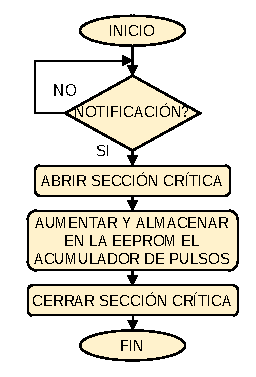
\includegraphics[scale=1]{./Figures/data_logger_pulses.pdf}
	\caption{Diagrama flujo de la tarea para el registro de pulsos de DATA LOGGER.}
		\label{fig:flowDataPulses}
\end{figure}

Según el diagrama de flujo de la figura \ref{fig:flowDataPulses}, la tarea de registro de pulsos espera por una notificación provocada por el flanco de subida de los pulsos eléctricos del medidor. Cuando esto ocurre, se abre una sección crítica para prevenir que existan cambios de contexto dentro del sistema operativo que modifiquen los datos implicados antes de que estos puedan ser utilizados. Una vez en la sección crítica, en una variable de 16 bits se acumulan la cantidad de pulsos detectados y se almacenan en la EEPROM en una dirección de memoria definida por una variable que hace referencia al índice. Finalmente, se cierra la sección crítica y este proceso se lleva a cabo mientras el dispositivo funcione.

\begin{figure}[h]
	\centering
	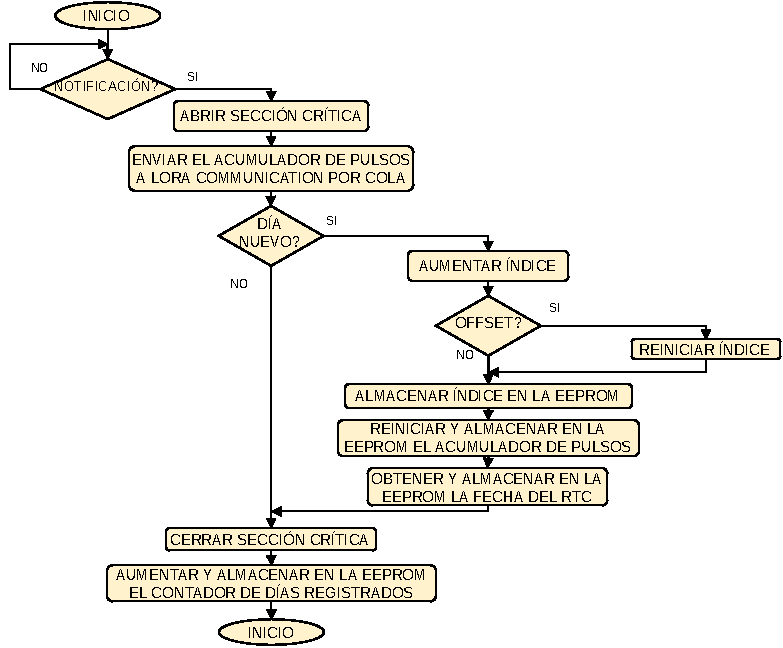
\includegraphics[scale=1]{./Figures/data_logger_alarm.pdf}
	\caption{Diagrama de flujo de la tarea que maneja las alarmas del RTC de DATA LOGGER.}
		\label{fig:flowDataAlarm}
\end{figure}

En el diagrama de la figura \ref{fig:flowDataAlarm}, los pulsos eléctricos generados por el RTC crean una notificación a la tarea que maneja las alarmas. Si se detecta una notificación, se abre una sección crítica donde mediante una cola se envía el valor de la variable acumuladora de pulsos al módulo LORA COMMUNICATION. Con ayuda del RTC, si se detecta un cambio de fecha, se ejecutan instrucciones para que la cantidad de pulsos contada a partir de ese momento se reinicie y se almacene en un posición diferente de la EEPROM, lo que evita que los datos en esta memoria se sobrescriban mientras exista espacio suficiente para almacenar más información. Si no se detecta un cambio en la fecha o en caso contrario, se ejecutó todo el proceso antes descrito para la modificación del índice de la EEPROM, el proceso termina, pero, vuelve a repetirse cada vez que ocurre una nueva notificación.

Para que este módulo funcione correctamente cuando el dispositivo es encendido se ejecuta una función de inicialización. En el diagrama de flujo de la figura \ref{fig:flowDataInit} se ilustra su comportamiento.

\begin{figure}[h]
	\centering
	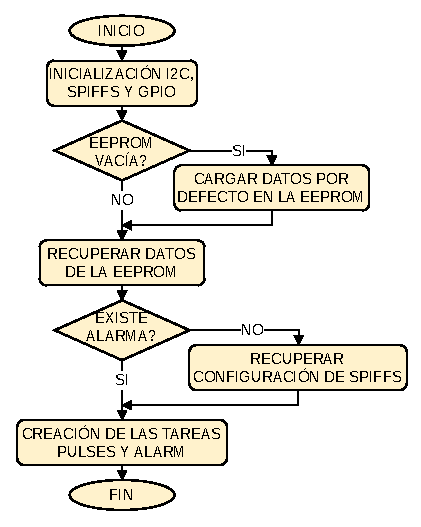
\includegraphics[scale=1]{./Figures/data_logger_init.pdf}
	\caption{Diagrama de flujo de la función de inicialización de DATA LOGGER.}
		\label{fig:flowDataInit}
\end{figure}

El procedimiento de inicialización del módulo, empieza con la configuración de los módulos I\textsuperscript{2}C, GPIO y SPIFFS para poder utilizar sus funciones. Se hace una lectura de la EEPROM para verificar si esta tiene datos de un funcionamiento anterior para almacenar los datos por defecto. Se recuperan los datos previamente cargados y se configura la alarma del RTC con los datos obtenidos de un archivo de texto almacenado en SPIFFS. Finalmente, se crean las tareas para acumular pulsos y manejar las alarmas.

\subsection{LORA COMMUNICATION}	

La función de este módulo se basa en utilizar el transceptor LoRa para intercambiar información con un dispositivo concentrador de datos de la misma tecnología. Sus tareas principales son enviar la cantidad de pulsos registrados y recibir parámetros de funcionamiento. Para esto, se comunica con otros módulos de las capas inferiores como se muestra en la figura \ref{fig:loraDiagram}.

\begin{figure}[h]
	\centering
	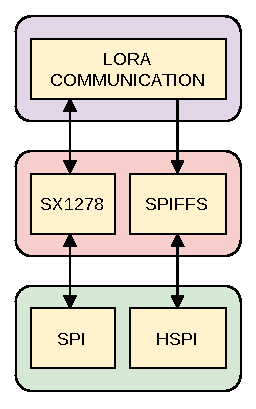
\includegraphics[scale=1]{./Figures/lora_communication_diagram.pdf}
	\caption{Diagrama de capas para LORA COMMUNICATION.}
		\label{fig:loraDiagram}
\end{figure}

Para que este módulo pueda enviar o recibir información utiliza las funciones proporcionadas por LORA a través del protocolo SPI para cambiar su modo de operación. Cuando recibe información del dispositivo concentrador de datos se accede a SPIFFS para modificar el archivo config.txt, lo que actualiza los parámetros de funcionamiento del dispositivo.

Este módulo posee una solo tarea que se ejecuta en el sistema operativo. En la figura \ref{fig:loraTask} puede observarse su comportamiento mediante un diagrama de flujo.

\begin{figure}[h]
	\centering
	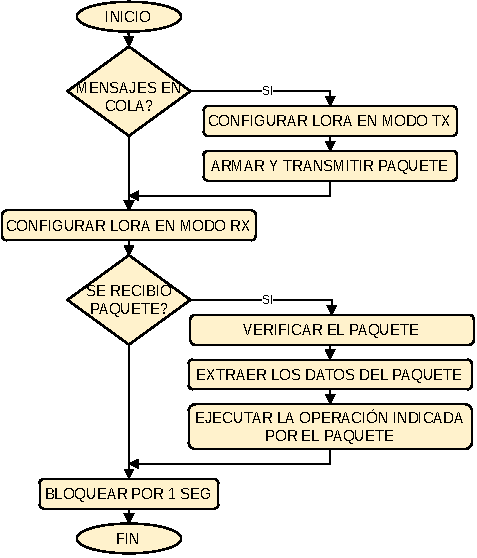
\includegraphics[scale=1]{./Figures/lora_communication_task.pdf}
	\caption{Diagrama de flujo de la tarea de la tarea transmisora y receptora de datos de LORA COMMUNICATION.}
		\label{fig:loraTask}
\end{figure}

Del diagrama de la figura \ref{fig:loraTask}, esta tarea consulta la cola de mensajes para determinar si existe algun elemento pendiente de atención. Si existen mensajes pendientes en la cola se configura el transceptor LoRa en modo de transmisión, se arma un paquete con la información necesaria y se envía. Si cola está vacía o se envió un paquete anteriormente, se configura el transceptor LoRa en modo de recepción y cuando se recibe un paquete se ejecuta la acción requerida por este. Finalizado todo este proceso la tarea se bloquea por un segundo y vuelve a repetirse mientras el dispositivo este en funcionamiento.

El formato de los paquetes enviados es el que se muestra en la figura \ref{fig:loraTxPacket}. Donde KEY e ID son campos de 32 bits que son obtenidos del archivo config.txt en SPIFFS, y representan la clave e identificador del usuario del dispositivo, respectivamente. KWH es un campo de 16 bits que representa el consumo eléctrico expresado en kWh. Por último, CRC es el campo para la redundancia cíclica y es de 8 bits.
\begin{figure}[h]
	\centering
	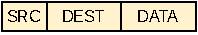
\includegraphics[scale=1]{./Figures/lora_communication_tx_packet.pdf}
	\caption{Formato de los paquete enviados.}
		\label{fig:loraTxPacket}
\end{figure}

Los paquete recibidos también tiene un formato y es el que se ilustra en la figura \ref{fig:loraRxPacket}. El campo KEY es la clave única del dispositivo y tiene un tamaño de 32 bits. OP es de 8 bits y define las operaciones que solicitadas al dispositivo, dichas operaciones pueden ser la modificación del archivo config.txt, configuración de la hora y fecha, solicitud de los datos de la EEPROM, por citar algunos. PARAM1 y PARAM2 son campos de 32 bits que contienen los parámetros con los que se deben ejecutar las operaciones requeridas por el campo OP. Finalmente, CRC es de 8 bits y tiene el valor de la redundancia cíclica.

\begin{figure}[h]
	\centering
	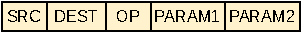
\includegraphics[scale=1]{./Figures/lora_communication_rx_packet.pdf}
	\caption{Formato de los paquete recibidos.}
		\label{fig:loraRxPacket}
\end{figure}

Este módulo tiene una función de inicialización que debe ser ejecutada cuando el dispositivo es energizado y el ESP8266 empieza a ejecutar el código que tiene grabado. Su comportamiento se muestra en el diagrama de flujo presentado en la figura \ref{fig:loraInit}

\begin{figure}[h]
	\centering
	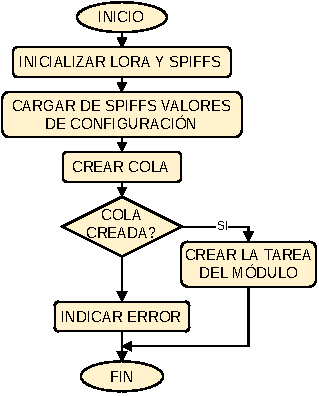
\includegraphics[scale=1]{./Figures/lora_communication_init.pdf}
	\caption{Diagrama de flujo de la función de inicialización del módulo LORA COMMUNICATION.}
		\label{fig:loraInit}
\end{figure}

Esta función de inicialización ejecuta todos los procesos necesarios para configurar el transceptor LoRa antes de utilizarlo. Posteriormente, intenta crear una cola para recibir información del módulo DATA LOGGER, si esta no puede ser creada termina la función e indica un error. Finalmente, si el proceso anterior se realizó exitosamente se crea la tarea que deberá ejecutarse para transmitir y recibir paquetes. 

\subsection{WEB SERVER}

El objetivo de este módulo es establecer un servidor web con la capacidad de conectarse con dispositivos que dispongan de conexión Wi-Fi, para permitirles leer o modificar el contenidos del sistema de archivos. Para cumplir con lo planteado anteriormente, se utilizan los componentes de las capas inferiores como indica la figura \ref{fig:serverDiagram}.

\begin{figure}[h]
	\centering
	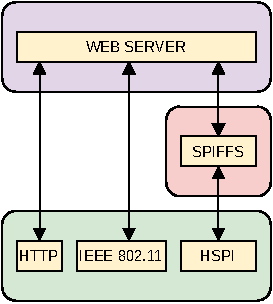
\includegraphics[scale=1]{./Figures/web_server_diagram.pdf}
	\caption{Diagrama de capas para WEB SERVER.}
		\label{fig:serverDiagram}
\end{figure}

Web Server utiliza las funciones del módulo HTTP para establecer un servidor que puede comunicarse con múltiples clientes HTTP mediante los métodos GET y POST, para la transferencia y modificación de los archivos almacenados en SPIFFS. El módulo IEEE 802.11 proporciona funciones para que WEB SERVER configure todas las funciones disponibles del transceptor Wi-Fi del ESP8266.

WEB SERVER puede configurar el dispositivo como punto de acceso o como estación, esto se hace de manera automática y depende de la información guardada en el archivo config.txt. En cualquiera de los dos modos citados los clientes pueden acceder al servidor a través de su dirección de red como indican las figuras \ref{fig:serverAP} y \ref{fig:serverSTA}.                                                                                                                                                                                                                                                                                                                                                                                                                                                                                                                                                                                                                                                                                                                                                                                                                                                                                                                                                                                                                                                                          

\begin{figure}[h]
	\centering
	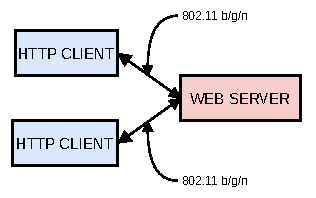
\includegraphics[scale=1]{./Figures/web_server_ap.pdf}
	\caption{WEB SERVER en modo punto de acceso.}
		\label{fig:serverAP}
\end{figure}

\begin{figure}[h]
	\centering
	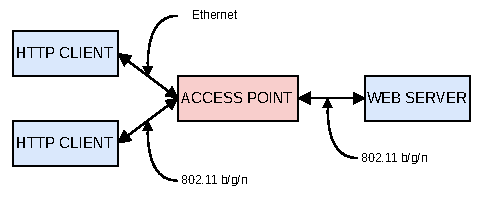
\includegraphics[scale=1]{./Figures/web_server_sta.pdf}
	\caption{WEB SERVER en modo estación.}
		\label{fig:serverSTA}
\end{figure}

En la figura \ref{fig:serverAP}, el dispositivo está configurado en modo punto de acceso y el servidor web puede ser accedido directamente por un cliente HTTP que cuente con conectividad Wi-Fi. Por otro lado, en la figura \ref{fig:serverSTA} el dispositivo está configurado en modo estación y los clientes HTTP solo podrán acceder a este a través de un punto de acceso con conectividad Wi-Fi que enrute las conexiones.

WEB SERVER tiene la capacidad de responder a peticiones GET y POST provenientes de los clientes HTTP gracias a una tarea que se ejecuta todo el tiempo en el sistema operativo. El método GET es utilizado para solicitar los archivos necesarios para generar la interfaz web, mientras que el método POST se utiliza para modificar el archivo config.txt del sistema de archivos. Para esto, WEB SERVER utiliza funciones que se ejecutan para transferir los recursos cuyo nombre coinciden con la URI (\textit{Uniform Resource Identifier, identificador de recursos uniforme}) en caso del método GET. En el caso del método POST se lee el cuerpo del mensaje recibido para extraer los parámetros con los que debe ser modificado config.txt y actualizar la información de conexión de red Wi-Fi.

Como los módulos Data Logger y Lora Communication, Web Server también posee una función de inicialización que configura todos los módulos de capas inferiores de los que depende, para que pueda cumplir su propósito. El diagrama de flujo de la figura \ref{fig:serverInit} es utilizado para explicar su funcionamiento.

\begin{figure}[h]
	\centering
	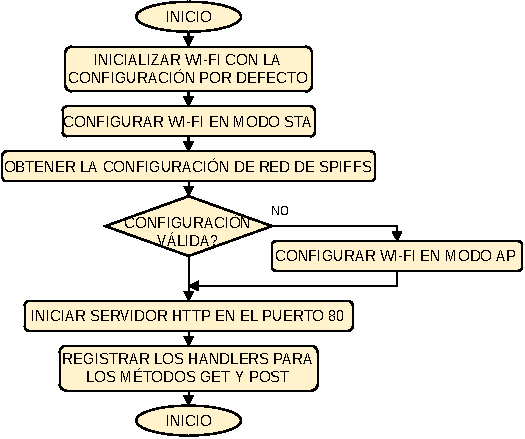
\includegraphics[scale=1]{./Figures/web_server_init.pdf}
	\caption{Diagrama de flujo de la función de inicialización del módulo WEB SERVER.}
		\label{fig:serverInit}
\end{figure}

En esta función el primer paso es inicializar la interfaz física de Wi-Fi con la configuración por defecto del ESP8266. Se configura el dispositivo en modo estación y se busca en el archivo config.txt configuración de red que permita conectarse a una red Wi-Fi existente. Si no existe dicha información o es inválida, se configura el dispositivo en modo punto de acceso. En cualquiera de los dos casos el siguiente paso es iniciar un servidor HTTP en el puerto 80 y finalmente registrar todas las funciones para los métodos GET y POST.

%----------------------------------------------------------------------------------------

\section{Interfaz web}

El diseño e implementación de una interfaz web, tiene como objetivo proporcionar a los usuarios, es decir, a los abonados de las compañías eléctricas, la capacidad de interactuar con el dispositivo para visualizar gráficamente información relativa a su consumo eléctrico y configurar parámetros de la conexión Wi-Fi.

Para el desarrollo se utilizo el IDE Visual Studio Code, que ofrece un entorno de desarrollo muy intuitivo y también brinda la posibilidad de descargar \textit{plugins} que facilitan la escritura de código. Asimismo, se utilizaron distintos lenguajes enfocados en el desarrollo web, para brindar a la interfaz una estructura bien definida, estética y funcionalidad. Estos fueron:

\begin{itemize}
	\item HTML: se utilizó para definir todos los aspectos estructurales de la interfaz, como la ubicación de los elementos, las llamadas a bibliotecas externas y otros parámetros informativos. La versión utilizada fue HTML 5.
	\item CSS: brindó control sobre la presentación, formato y el diseño de la interfaz.
	\item JavaScript: permitió dotar de funcionalidad a los elementos de la interfaz. Fue necesaria para realizar el procesamiento de los datos provenientes del dispositivo.
	\item jQuery Mobile: con esta biblioteca fue posible darle a la interfaz un aspecto de aplicación para teléfonos móviles, además de la capacidad de adaptarse a cualquier tamaño de pantalla sin que la información mostrada se vea alterada.
	\item Highcharts: a través de esta biblioteca se logró exhibir la información de consumo eléctrico en un gráfico de barras, de esta manera era más comprensible para el usuario.\end{itemize}

La interfaz web está dividida en dos pantallas, principal y de configuración. La primera es meramente informativa y es donde se muestra el consumo eléctrico al usuario. La segunda permite conectar el dispositivo a un red Wi-Fi existente.

La pantalla principal fue diseñada pensando en brindarle al usuario la información de su consumo eléctrico de la manera más simple posible. En la mayor parte del área de la pantalla se muestra un gráfico de barras que presenta el consumo eléctrico de los últimos tres meses y en la esquina superior izquierda un pequeño botón que dirige a la pantalla de configuración.

Al cargar la interfaz en un navegador web, se obtiene mediante el método GET el archivo pulses.csv que contiene los valores de consumo eléctrico que están almacenados en el dispositivo. Estos son procesados con instrucciones escritas en JavaScript para que la biblioteca Highcharts los utilicé y genere el gráfico de barras. En la figura \ref{fig:interfaceMain} se observa la pantalla principal de la interfaz web.

\begin{figure}[h]
	\centering
	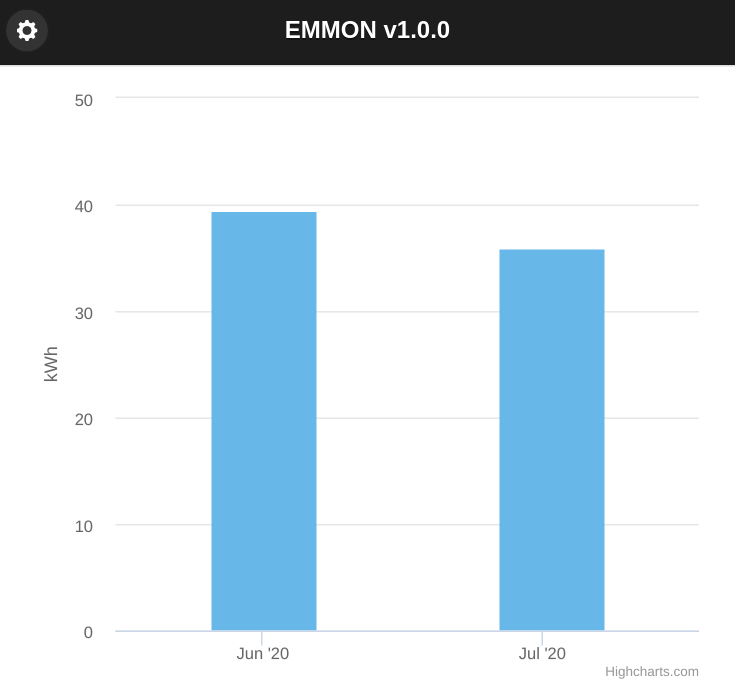
\includegraphics[scale=0.3]{./Figures/interface_main.png}
	\caption{Pantalla principal de la interfaz web.}
	\label{fig:interfaceMain}
\end{figure}

Se diseño la pantalla de configuración para que la única configuración que puede realizarse sea la conexión del dispositivo a una red Wi-Fi existente a través de su SSID y contraseña. Esta pantalla es imprescindible, debido a que el dispositivo no debería ser manipulado manualmente bajo ninguna circunstancia por el usuario y se necesitaba una forma de realizar esta configuración.

El componente principal es un formulario para ingresar el SSID y contraseña de la red a la que el usuario desea conectar el dispositivo. En la esquina superior izquierda se encuentra un botón para retornar a la pantalla principal y en la esquina superior derecha un botón para enviar por el método POST el contenido del formulario al dispositivo. En la figura \ref{fig:interfaceConf} se muestra la pantalla de configuración de la interfaz web.

\begin{figure}[h]
	\centering
	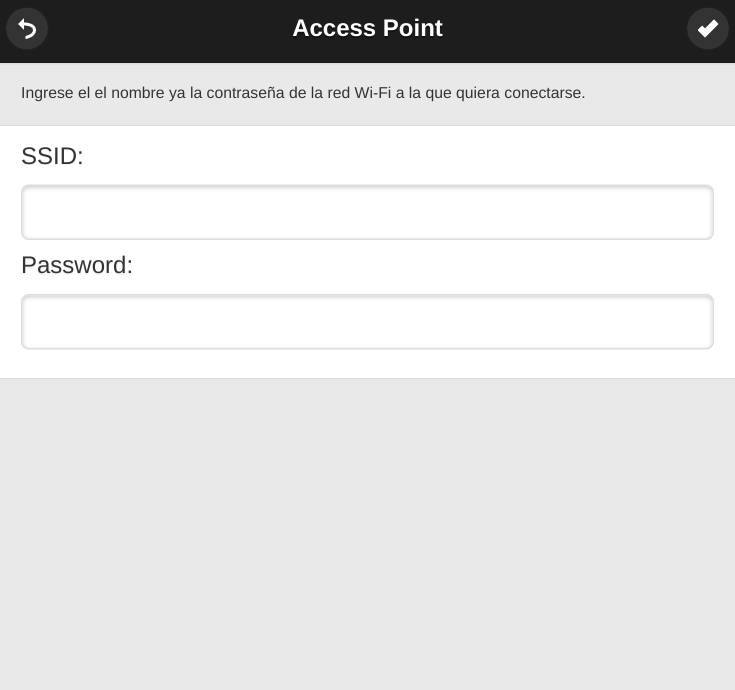
\includegraphics[scale=0.3]{./Figures/interface_conf.png}
	\caption{Pantalla de configuración de la interfaz web.}
	\label{fig:interfaceConf}
\end{figure}
%----------------------------------------------------------------------------------------

\section{Prototipo comercial}

El desarrollo de un prototipo para ser comercializado, fue necesario para una primera implementación del dispositivo en un entorno real de trabajo y la realización de pruebas a nivel físico. El mismo consta de una carcasa y un PCB (\textit{Printed Circuit Board}, tarjeta de circuito impreso).

El primer paso, fue elegir una carcasa de dimensiones adecuadas para que pueda ser montada directamente sobre un medidor de consumo eléctrico domiciliario. Para este fin, se estudió la posibilidad de diseñar una carcasa personalizada, pero, debido a los altos costos de producción a nivel de prototipo, esta idea fue rápidamente descartada. Entonces, después de realizar un análisis de las dimensiones de los medidores utilizados por COPELECT, se eligió una carcasa disponible en el mercado internacional, la VG-S43 de la firma Vange. La elección de esta carcasa sobre otras similares, fue debido a los zócalos que tenía, que se adecuaban perfectamente para que el fototransistor estuviera descubierto y tuviera vista directa con el LED del medidor eléctrico. En la figura \ref{fig:case} se puede apreciar el carcasa elegida.

\begin{figure}[h]
	\centering
	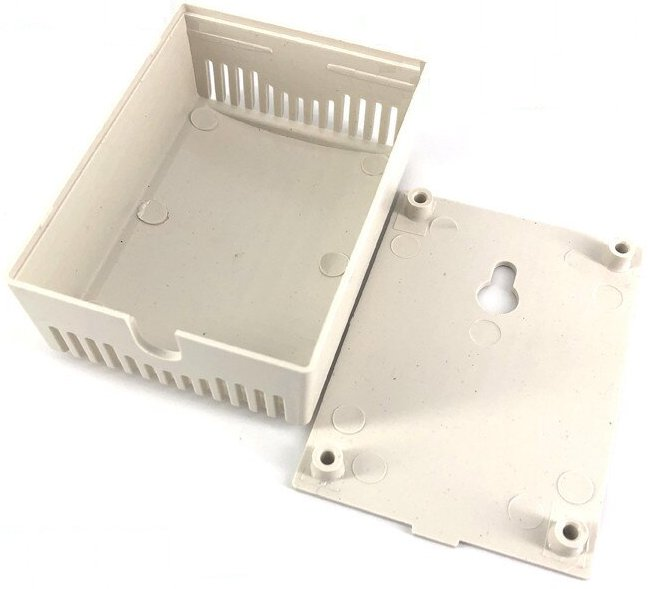
\includegraphics[scale=0.4]{./Figures/case.jpg}
	\caption{Carcasa VG-S43 de la firma Vange\protect\footnotemark.}
		\label{fig:case}
\end{figure}

	\footnotetext{Imagen tomada de: \url{https://es.aliexpress.com/item/33004284623.html?spm=a2g0o.cart.0.0.50483c00xuS0Xo&mp=1}}

Antes de empezar con el diseño del PCB, se realizó la elección de los componentes que serían parte del mismo. En el prototipo de pruebas se utilizaron módulos y tarjetas de desarrollo que con el firmware implementado en ellos, cumplieron todos los requerimientos planteados. Entonces, para que el firmware desarrollado pudiera ser utilizado exitosamente en el prototipo comercial, se utilizaron los circuitos integrados principales de los módulos y tarjetas de desarrollo, también se descartaron los componentes electrónicos que no resultaban necesarios para este trabajo. Existen dos componentes que se implementaron como módulos, el ESP-12F que es componente principal de la NodeMCU, y el RA-01, que es un transceptor LoRa basado en el mismo circuito integrado que el PM1280, el SX1278. Además, el PT333-3C fue sustituido por el PT11-21C, que también es un fototransistor de similares características, pero es un SMD (\textit{Surface-Mount-Device}, dispositivo de montaje superficial).

Una vez elegidos los componentes implicados, se realizó un análisis del consumo de corriente de cada uno de ellos, para implementar una fuente de alimentación adecuada. Cabe resaltar que el voltaje de alimentación de de todos los componentes es 3,3 V. En la tabla x se muestran los valores máximos de consumo de corriente de los componentes, estos datos fueron obtenidos de los \textit{datasheets} de los mismos.

\begin{table}[h]
	\centering
	\caption[Consumo del prototipo comercial]{Tabla de consumo eléctrico de los componentes del prototipo comercial}
	\begin{tabular}{l c}    
		\toprule
		\textbf{Componente} & \textbf{Consumo de corriente (mA)} \\
		\midrule
		ESP-12F 	& 500 (en modo de transmisión continua) \\		
		RA-01		& 93 (en modo transmisor)\\
		DS3231		& 0,2 (en modo activo) \\
		AT24C32 	& 3 (cuando se escribe un dato)\\
		LM393 		& 20 (cortocircuitado a tierra) \\
		PT11-21C	& 20 \\
		\bottomrule
		\hline
	\end{tabular}
	\label{tab:componentsPower}
\end{table}

De la tabla anterior, se determinó que el consumo total de todos los componentes es de 636,2 mA. Al momento de elegir la fuente de alimentación al consumo total se le añadió un margen de seguridad del 50\%, dando un nuevo valor de 954,43 mA. Por lo tanto, la fuente de alimentación elegida debió ser de 3.3 V y 1 A.

Para reducir la cantidad de componentes de la fuente de alimentación, se escogió un módulo conversor de energía alterna a directa. De esta forma, el prototipo comercial podría conectarse directamente a la misma línea eléctrica del medidor. El componente elegido fue el módulo HLK-PM03 de la firma Hi-Link, que proporciona 3,3 V y 1 A a su salida, cuando a la entrada existen 90 V - 240 V alternos. En la figura \ref{fig:powerModule} puede observarse el módulo para la fuente de alimentación.

\begin{figure}[h]
	\centering
	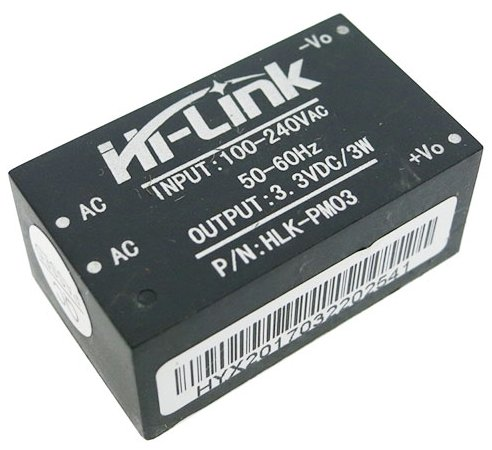
\includegraphics[scale=0.3]{./Figures/acdc_module.jpg}
	\caption{Módulo de alimentación HLK-PM03 de la firma Hi-Link\protect\footnotemark.}
		\label{fig:powerModule}
\end{figure}

	\footnotetext{Imagen tomada de: \url{https://es.aliexpress.com/item/33004284623.html?spm=a2g0o.cart.0.0.50483c00xuS0Xo&mp=1}}
	
Con ayuda del software KiCAD, se realizó el dibujo de un diagrama esquemático del prototipo comercial, que interconecta todos los componentes y brinda información relacionada a aspectos importantes sobre el funcionamiento y diseño del PCB. En la figura \ref{fig:schematic} se muestra el diagrama esquemático del prototipo comercial.

\begin{figure}[h]
	\centering
	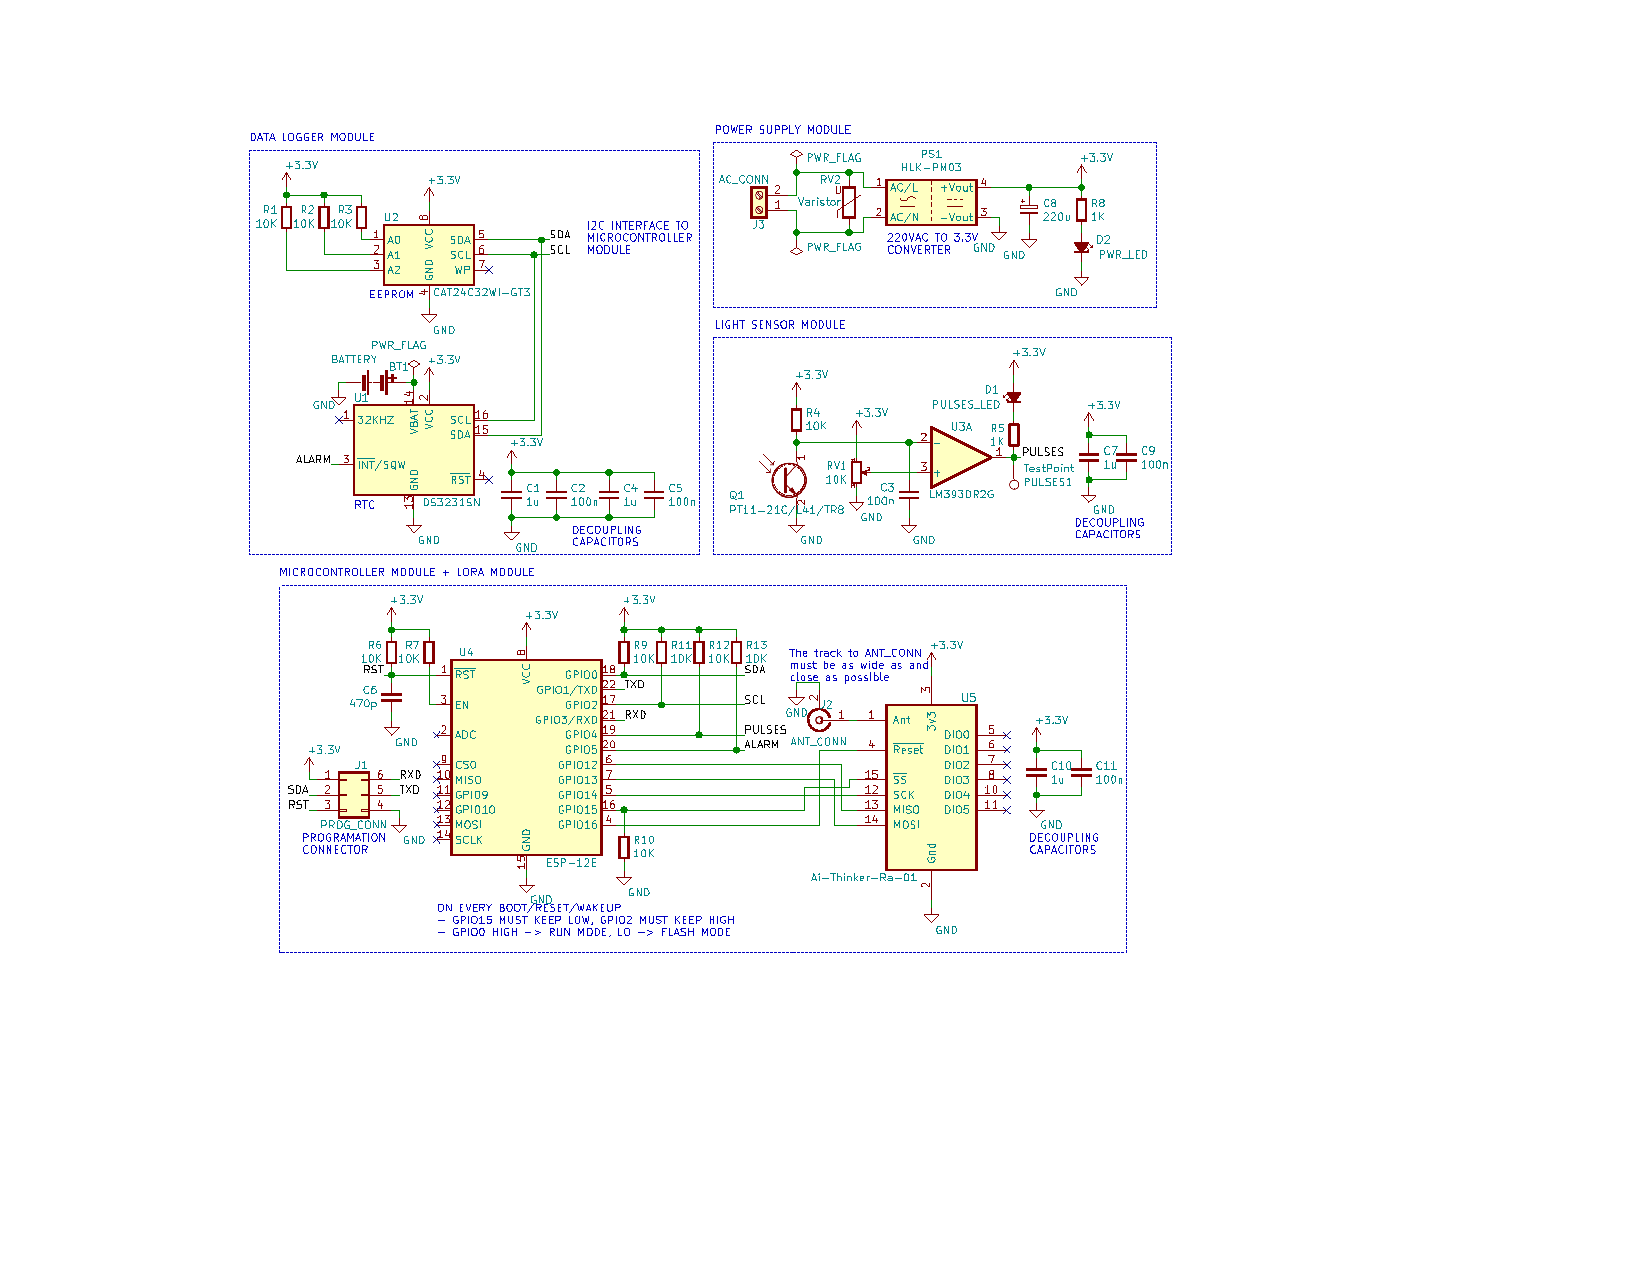
\includegraphics[scale=0.9]{./Figures/schematic.pdf}
	\caption{Diagrama esquemático del prototipo comercial.}
		\label{fig:schematic}
\end{figure}

Del diagrama anterior, se puede notar que se añadieron \textit{test points} para poder probar la respuesta del sensor de luz mediante instrumentación especializada. Se añadieron también, un conector destinado a la depuración del código almacenado en el ESP8266, junto con LEDs para monitorear el estado de la fuente y el sensor de luz.

Con el diagrama esquemático finalizado, se realizó la ERC (\textit{Electrical Rule Check}, comprobación de reglas eléctricas) en busca posibles cortocircuitos, conexiones ilegales y contactos flotantes entre otras comprobaciones. Posteriormente, se dibujó el circuito impreso, donde se tuvieron en consideración las restricciones físicas impuestas por la elección de la carcasa. Se tuvo especial énfasis en la ubicación de los conectores, para que estos quedaran al borde del PCB y pudieran ser accedidos con mayor facilidad. El fototransistor quedó ubicado en una posición tal que coincidiera con el zócalo inferior de la carcasa. Otra consideración de importancia fue la distancia entre el transceptor LoRa y el conector coaxial, ambos componentes fueron ubicados muy cerca, de tal forma que la pista que los conectaba tuviera una distancia muy corta, asimismo, se dibujo la pista lo más ancha posible y se pusieron vías conectadas a tierra para lograr una mejor respuesta a las interferencias electromagnéticas.

Las capas \textit{top} y \textit{bottom} del PCB, pueden apreciarse en las figuras \ref{fig:pcbTop} y \ref{fig:pcbBot}, respectivamente. Por otro parte, en las figuras \ref{fig:pcb3D} y \ref{fig:pcbReal}, se muestran el modelo 3D renderizado del PCB y una fotografía del PCB montado.

\begin{figure}[h]
	\centering
	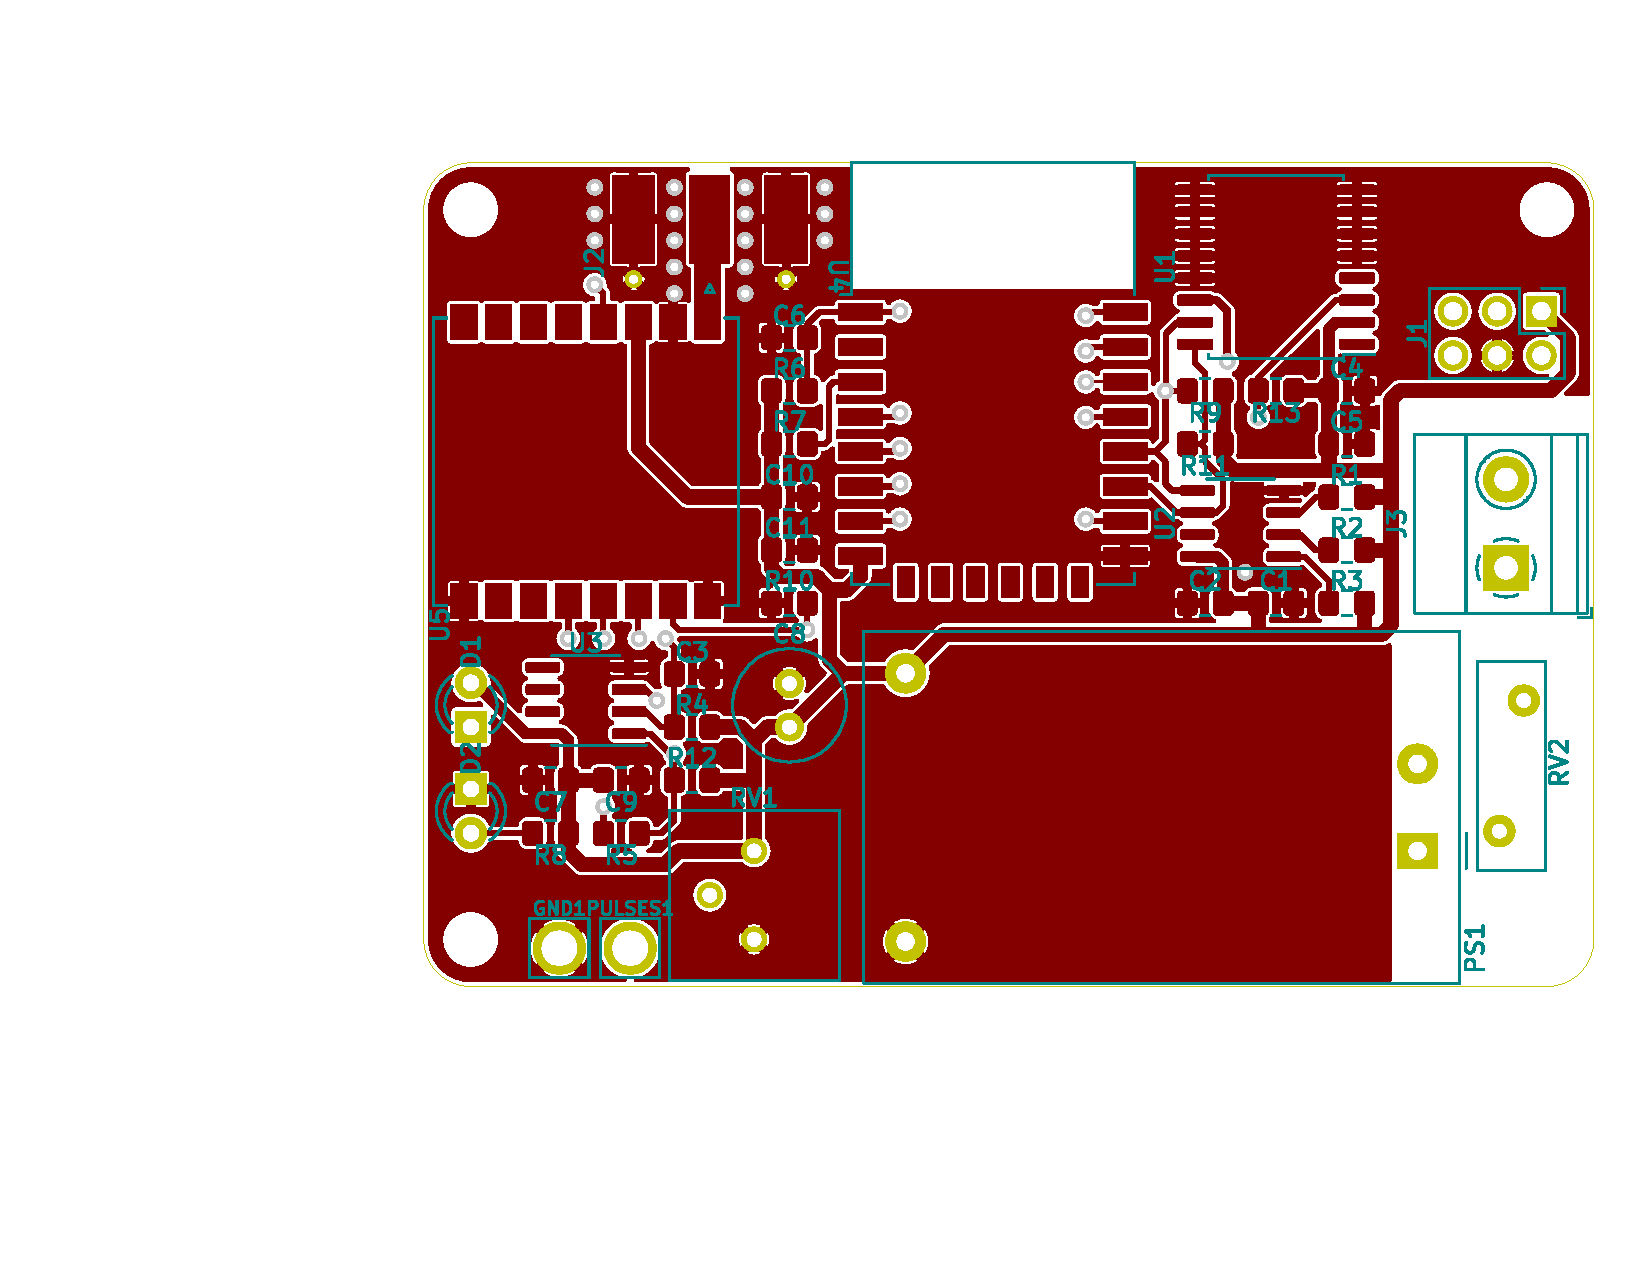
\includegraphics[scale=0.5]{./Figures/pcb_top.pdf}
	\caption{Capa top del PCB.}
		\label{fig:pcbTop}
\end{figure}

\begin{figure}[h]
	\centering
	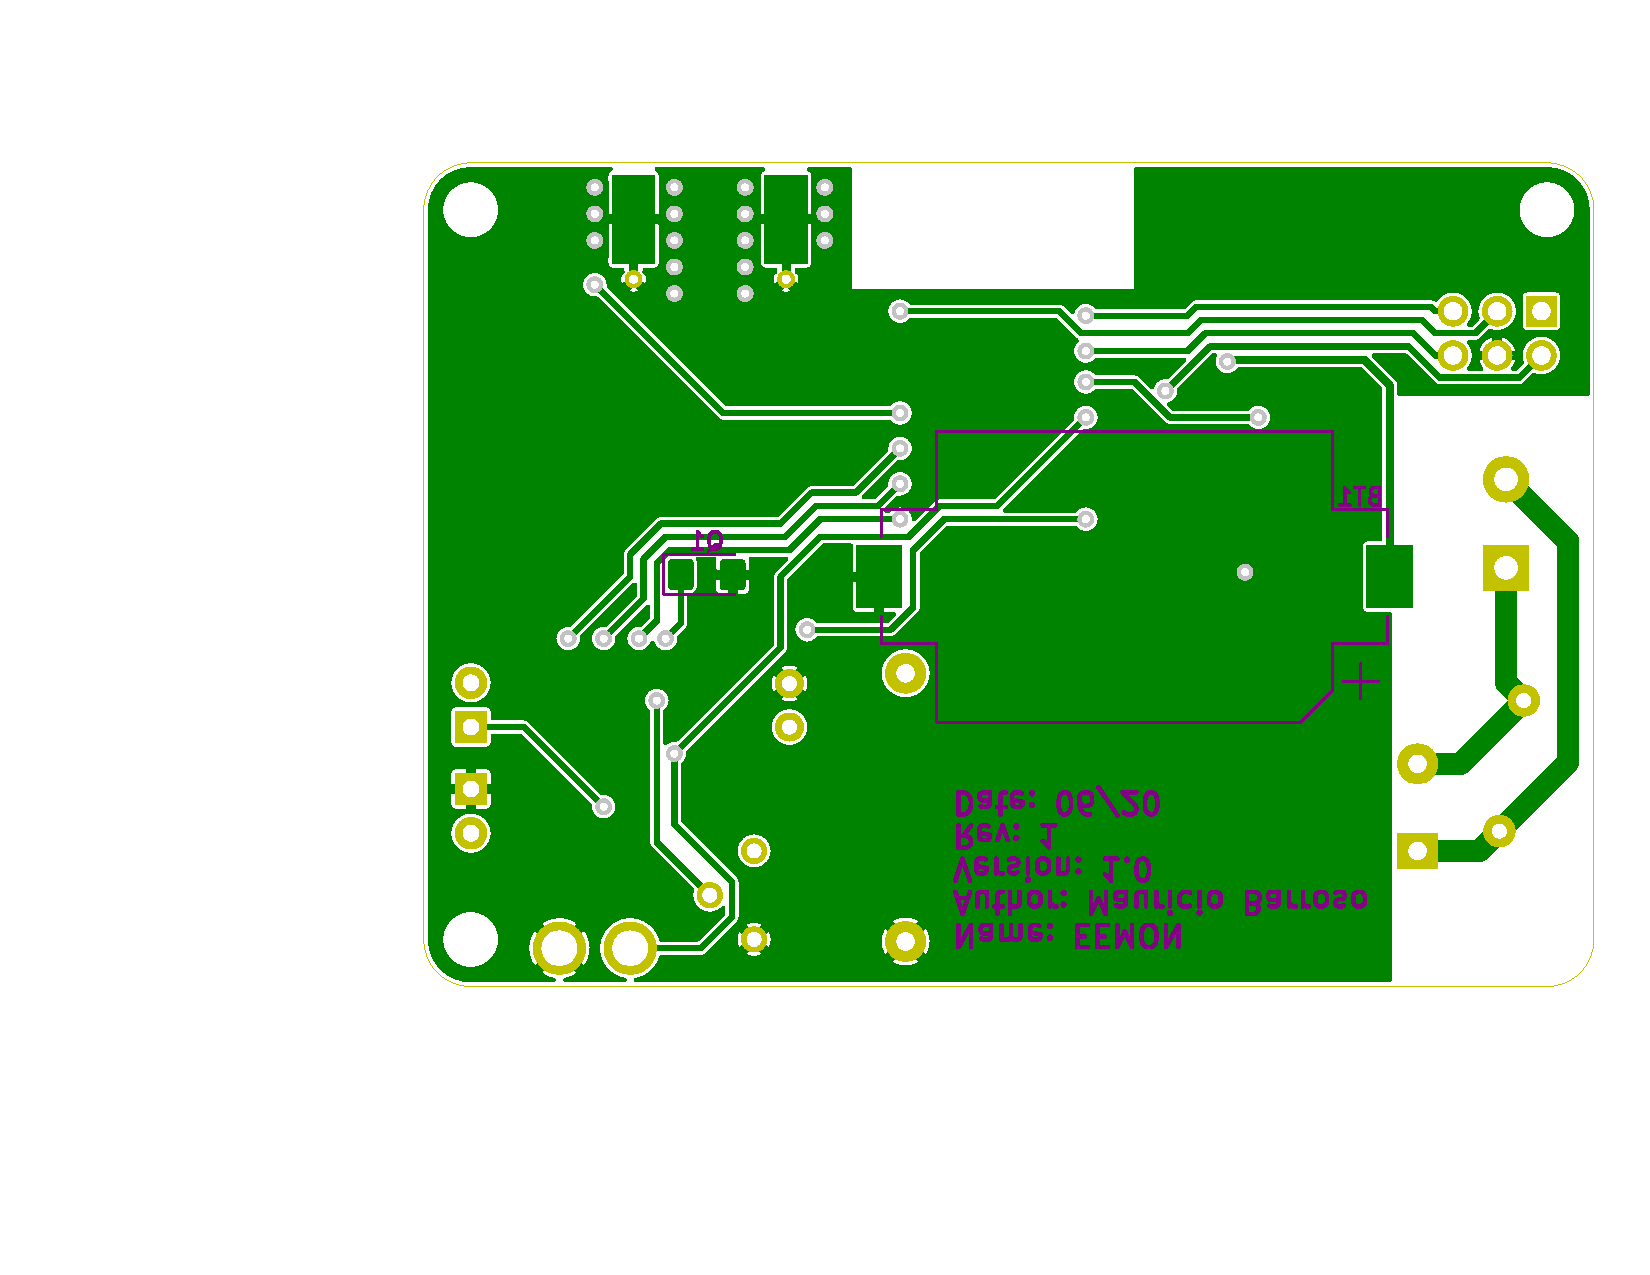
\includegraphics[scale=0.5]{./Figures/pcb_bot.pdf}
	\caption{Capa bottom del PCB.}
		\label{fig:pcbBot}
\end{figure}

\begin{figure}[h]
	\centering
	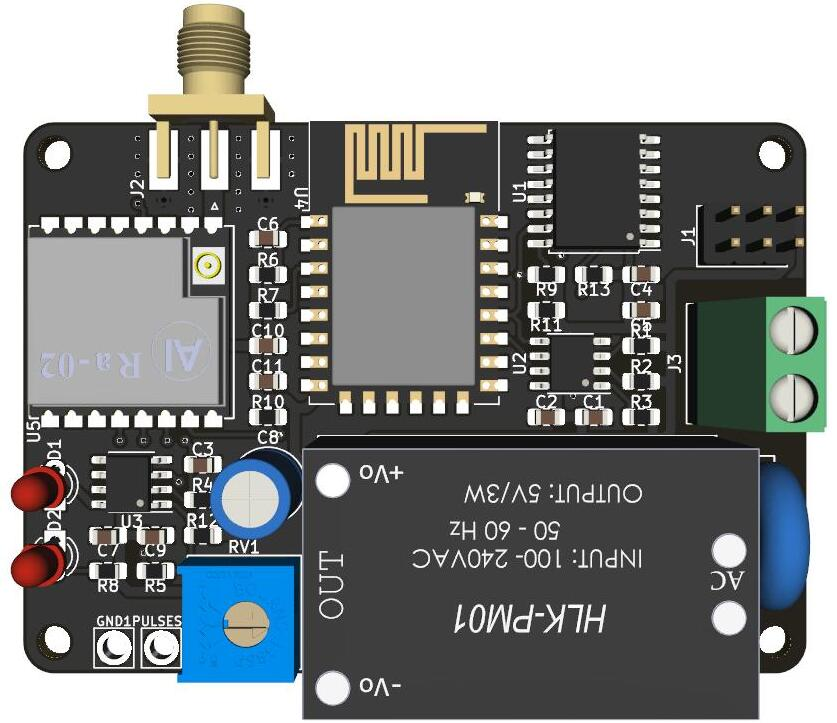
\includegraphics[scale=0.375	]{./Figures/pcb_3d.jpg}
	\caption{Modelo 3D del PCB montado del prototipo comercial.}
		\label{fig:pcb3D}
\end{figure}

\begin{figure}[h]
	\centering
	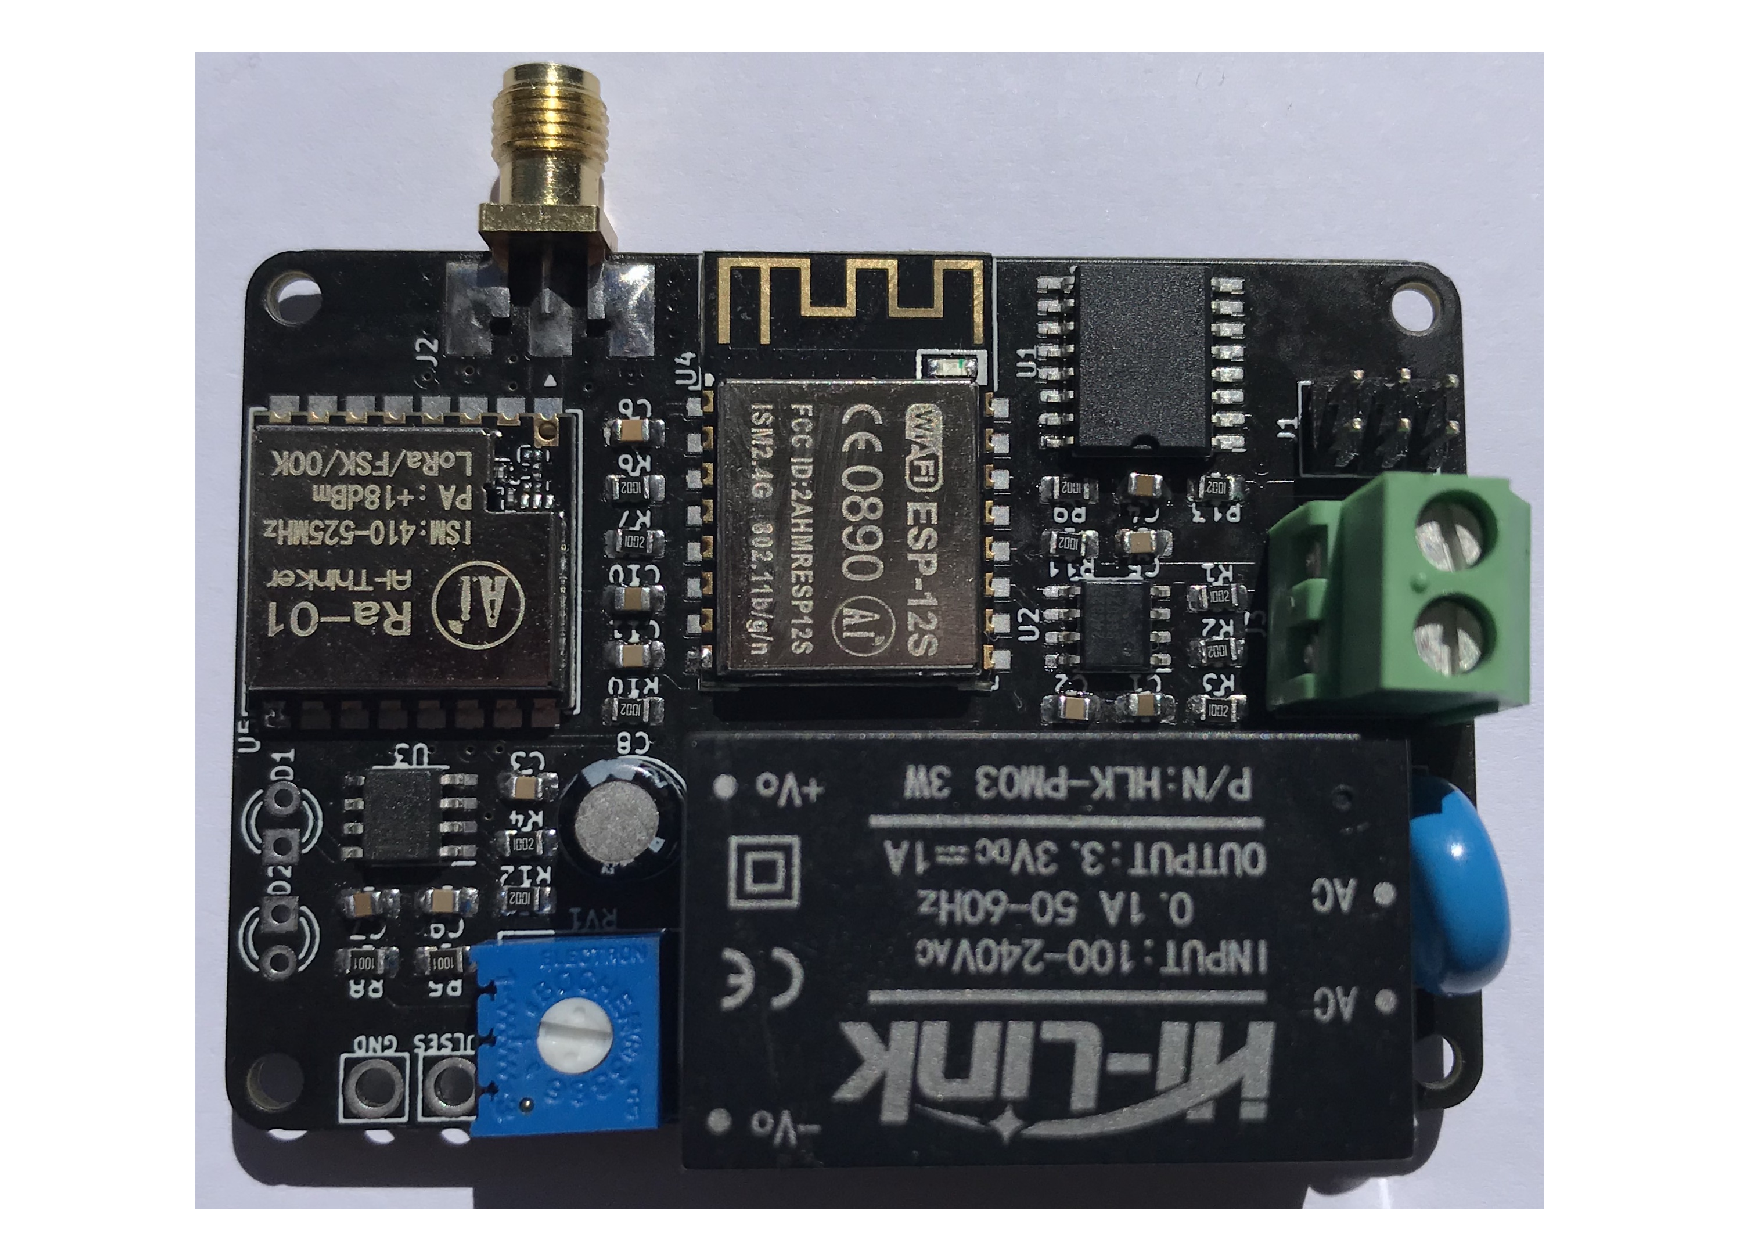
\includegraphics[scale=0.5	]{./Figures/pcb_real.pdf}
	\caption{PCB montado del prototipo comercial.}
		\label{fig:pcbReal}
\end{figure}

La manufactura del PCB fue realizada por el fabricante JLCPCB y los componentes fueron adquiridos de la firma LCSC. Ambos fueron elegidos por los costos reducidos que ofrecen en sus productos, además de que JLCPCB ofrece el servicio de PCBA (\textit{Printed Circuit Board Assembly}, montaje de PCB) con los componentes que tiene disponibles LCSC.
% Chapter Template

\chapter{Ensayos y resultados} % Main chapter title

\label{Chapter4} % Change X to a consecutive number; for referencing this chapter elsewhere, use \ref{ChapterX}

%----------------------------------------------------------------------------------------

%\section{Introducción}

En este capítulo se presentan los ensayos realizados sobre los prototipos de pruebas y comercial. Además se exhiben los resultados obtenidos que validan su correcto funcionamiento. Las pruebas fueron realizadas sobre el firmware y hardware expuestos en el capítulo \ref{Chapter3}.

%----------------------------------------------------------------------------------------

\section{Pruebas unitarias}
\label{sec:pruebasU}

Se hicieron pruebas unitarias sobre las bibliotecas desarrolladas para el manejo de los circuitos integrados DS3231, AT24C32 y SX1278. Se utilizó Ceedling para ejecutar dichas pruebas en combinación con Gcov para generar los análisis de cobertura correspondientes. En la tabla \ref{tab:resultsCeedling} se pueden observar los resultados de las pruebas unitarias y en la tabla \ref{tab:coverAnalysis} se exhibe el análisis de cobertura.

\begin{table}[h]
	\centering
	\caption[Pruebas unitarias]{Tabla de resultados de las pruebas unitarias.}
	\begin{tabular}{l c c c}    
		\toprule
		\textbf{Biblioteca} & \textbf{Cantidad de tests} & \textbf{Exitosos} & \textbf{Fallidos}  \\
		\midrule
		AT24C32 & 8	& 8 & 0 \\		
		DS3231 & 11 & 11 & 0 \\
		SX1278 & 14 & 14 & 0 \\
		\bottomrule
		\hline
	\end{tabular}
	\label{tab:resultsCeedling}
\end{table}

\begin{table}[h]
	\centering
	\caption[Análisis de cobertura]{Tabla de resultados del análisis de cobertura.}
	\begin{tabular}{l c c}    
		\toprule
		\textbf{Archivo} & \textbf{Líneas ejecutadas} & \textbf{Funciones ejecutadas}  \\
		\midrule
		at24c32.c & 52/52 & 6/6 \\		
		ds3231.c & 54/62 & 11/13 \\
		sx1278.c & 172/220 & 26/31 \\
		\bottomrule
		\hline
	\end{tabular}
	\label{tab:coverAnalysis}
\end{table}

%----------------------------------------------------------------------------------------

\section{Pruebas funcionales de firmware}
\label{sec:pruebasFW}

Se probaron los módulos DATA LOGGER, LORA COMMUNICATION y WEB SERVER de la capa superior del firmware, APP. Durante la etapa de desarrollo del firmware, estos módulos fueron probados para garantizar su correcto funcionamiento, de acuerdo con la planificación del trabajo descrita en el capítulo \ref{Chapter2}. El banco de pruebas utilizado consiste en el prototipo de pruebas conectado a una PC por medio de un cable micro USB. También se utilizó un medidor eléctrico modelo LUMEN 2 MC de la firma Nansen, que fue facilitado por COPELECT. El banco de pruebas se muestra en la figura \ref{fig:testFunctional}.

\begin{figure}[ht]
	\centering
	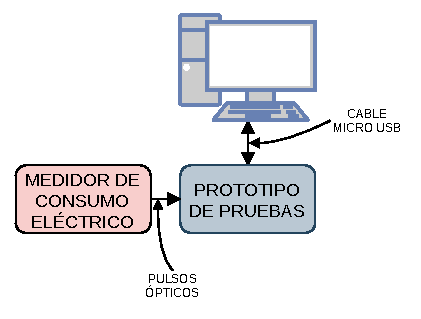
\includegraphics[scale=1.2]{./Figures/test_firmware_functional.pdf}
	\caption{Banco de pruebas para evaluar el funcionamiento del firmware.}
	\label{fig:testFunctional}
\end{figure}

Las pruebas consistieron en monitorear a través de la PC el funcionamiento de los módulos que componen la capa APP. Para esto, se añadieron instrucciones en el código fuente de estos módulos, que sirvieron para imprimir mensajes por el puerto serial. En la PC se ejecutó la utilidad idf-monitor, que es una terminal para puerto serial incluida en el ESP8266\_RTOS\_SDK. A medida que se desarrollaron los módulos, estos fueron probados individualmente verificando su correcto funcionamiento. 

Con todos los módulos funcionando individualmente, se realizó la prueba de integración de la capa APP. En la figura \ref{fig:testIDF1} se observa una captura de pantalla del idf-monitor cuando el dispositivo inicia su operación.

\begin{figure}[ht]
	\centering
	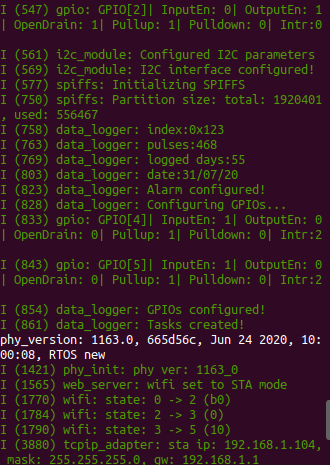
\includegraphics[scale=0.55]{./Figures/test_firmware_init.png}
	\caption{Captura de pantalla de idf-monitor cuando el dispositivo inicia.}
	\label{fig:testIDF1}
\end{figure}

Las funciones que se ejecutan en el sistema operativo del dispositivo también generaron mensajes informativos. En la captura de pantalla de la figura \ref{fig:testIDF2}, se observan los mensajes que imprimen las tareas de los módulos cuando funciona normalmente.

\begin{figure}[ht]
	\centering
	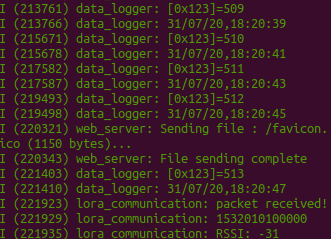
\includegraphics[scale=0.55]{./Figures/test_firmware_tasks.png}
	\caption{Captura de pantalla de idf-monitor cuando el dispositivo ejecuta sus funciones normales.}
	\label{fig:testIDF2}
\end{figure}

Con ayuda de todos los mensajes generados, además de los diagramas de flujo presentados en el capítulo \ref{Chapter3}, se pudo probar que los módulos de firmware del dispositivo funcionan correctamente.

%----------------------------------------------------------------------------------------

\section{Pruebas de la interfaz web}

Las pruebas realizadas sobre la interfaz web tuvieron la finalidad de corroborar su funcionalidad. De acuerdo a lo expuesto en el capítulo \ref{Chapter3}, el dispositivo puede ser configurado mediante el módulo WEB SERVER en dos modos de operación. Entonces, se realizaron dos tipos de pruebas distintas, una con el dispositivo como punto de acceso y la otra como estación. Para estas pruebas se utilizó una PC, un cable micro USB, un \textit{router} Wi-Fi TL-WR940N de la firme TP-Link y una \textit{laptop} con el navegador web Chrome instalado. En la figura \ref{fig:testInterface} se puede ver un diagrama del banco de pruebas montado.

\begin{figure}[ht]
	\centering
	\includegraphics[scale=1.1]{./Figures/test_interface_bank.pdf}
	\caption{Banco de pruebas para verificar el funcionamiento de la interfaz web cuando el dispositivo está en modo punto de acceso.}
	\label{fig:testInterface}
\end{figure}

El primer paso fue eliminar todas las configuraciones existentes en el sistema de archivos del dispositivo, lo que provocó que al iniciar se ejecutaran las instrucciones por defecto del mismo. Por defecto el dispositivo se configura como punto de acceso. Luego, se conectó la laptop a la red Wi-Fi del dispositivo. En la figura \ref{fig:testScreenNet} se observa la red Wi-Fi generada por el dispositivo en el administrador de redes de la laptop. 

\begin{figure}[ht]
	\centering
	\includegraphics[scale=0.53]{./Figures/test_interface_nets.png}
	\caption{Captura de pantalla de las redes Wi-Fi disponibles en la laptop.}
	\label{fig:testScreenNet}
\end{figure}

El siguiente paso fue ingresar a la dirección de red del dispositivo mediante el navegador web de la laptop, que dio como resultado la transferencia del archivo index.html. Este archivo HTML solicitó automáticamente al dispositivo mediante el método GET todos los elementos restantes para generar la interfaz web. Para verificar que las transferencias de estos archivos se hicieran correctamente, para el lado del prototipo de pruebas se utilizó el idf-monitor y para el lado de la laptop, se hizo uso de la herramienta de depuración del navegador. En las figuras \ref{fig:testScreenBrowserDebug} y \ref{fig:testScreenIDFTransfer}, se muestran capturas de pantalla de la utilidad de depuración del navegador y la salida del idf-monitor, respectivamente.

\begin{figure}[ht]
	\centering
	\includegraphics[scale=0.5]{./Figures/test_interface_chrome_ap.png}
	\caption{Captura de pantalla de la página principal de la interfaz web con la utilidad de depuración funcionando.}
	\label{fig:testScreenBrowserDebug}
\end{figure}

\begin{figure}[ht]
	\centering
	\includegraphics[scale=0.53]{./Figures/test_interface_idf_downloads.png}
	\caption{Captura de pantalla del idf-monitor después de enviar los archivos solicitados por el navegador web y el dispositivo en modo punto de acceso.}
	\label{fig:testScreenIDFTransfer}
\end{figure}

La siguiente prueba consistió en ingresar a la página de configuración de la interfaz web a través el botón ubicado en la esquina superior izquierda de la página principal. Ahí se llenó el formulario con los datos de la red Wi-Fi generada por el router, es decir, su SSID y su contraseña. Se utilizó el botón ubicado en la esquina superior derecha para enviar estos datos al prototipo de pruebas con el método POST. Con esta información el módulo WEB SERVER cambio la configuración al modo estación y pudo conectarse al router, que le proporcionó una dirección de red. Por último, la laptop también se conectó a la red del router y se utilizó el navegador web junto con la nueva dirección de red del prototipo de pruebas para solicitar los archivos de la interfaz web. En las figuras \ref{fig:testScreenWifiConf} y \ref{fig:testScreenIDFTransfer2}, se pueden observar una captura de pantalla con los campos del formulario llenados y la salida del idf-monitor, respectivamente.

\begin{figure}[ht]
	\centering
	\includegraphics[scale=0.5]{./Figures/test_interface_form.png}
	\caption{Captura de pantalla de la página de configuración de la interfaz web con la utilidad de depuración funcionando.}
	\label{fig:testScreenWifiConf}
\end{figure}

\begin{figure}[ht]
	\centering
	\includegraphics[scale=0.55]{./Figures/test_interface_idf.png}
	\caption{Captura de pantalla del idf-monitor después de configurar el dispositivo en modo estación con los datos enviados por la interfaz web.}
	\label{fig:testScreenIDFTransfer2}
\end{figure}

Al finalizar estas pruebas se pudo evidenciar el correcto funcionamiento de las dos páginas de la interfaz web. Asimismo, implícitamente se verificó que el módulo de firmware WEB SERVER respondía las peticiones con los métodos GET y POST según lo esperado.

%----------------------------------------------------------------------------------------
\section{Pruebas de laboratorio}

Estas pruebas tuvieron como objetivo principal utilizar instrumentación especializada para verificar el buen funcionamiento del conversor óptico-eléctrico y la fuente de alimentación. 

El propósito de la prueba del conversor óptico-eléctrico fue observar la forma de onda que genera, para implementar un algoritmo en el firmware que evitará la detección de pulsos falsos consecuencia de las características intrínsecas del LED del medidor de consumo eléctrico proporcionado por COPELECT. Para llevar a cabo esta prueba se utilizó un osciloscopio TDS2000C de la firma Tektronix, el prototipo comercial y el medidor proporcionado por COPELECT. El banco de pruebas puede observarse en el diagrama de la figura \ref{fig:testHWBankCOE}.

\begin{figure}[ht]
	\centering
	\includegraphics[scale=1.2]{./Figures/test_pulses_bank.pdf}
	\caption{Banco de pruebas para el conversor óptico-eléctrico.}
	\label{fig:testHWBankCOE}
\end{figure}

\begin{figure}[ht]
	\centering
	\includegraphics[scale=0.5]{./Figures/pulses_debounce.jpg}
	\caption{Salida de la pantalla del osciloscopio.}
	\label{fig:testHWPhoto}
\end{figure}

De la figura \ref{fig:testHWPhoto}, se puede observar que la forma de onda producida por el medidor tiene elementos que pueden ocasionar que el módulo DATA LOGGER registre erróneamente los pulsos y generar un reporte erróneo del consumo de energía eléctrica. Para solucionar esto, se implementó una función similar a la utilizada para detectar rebotes en los pulsadores en DATA LOGGER. Con esto se evitó en gran medida el error antes mencionado.

La prueba de la fuente de alimentación tuvo como propósito excitar este elemento con una fuente de tensión alterna, que simuló el comportamiento de la línea de alimentación cuando existen cambios en su valor nominal. Los elementos utilizados fueron una fuente de tensión alterna variable modelo 1653A de la firma BK precisión, un reóstato como carga variable y dos multímetros MUT-39 de la firma Truper. El banco de pruebas utilizado se ilustra en la figura \ref{fig:testHWBankPower}

\begin{figure}[ht]
	\centering
	\includegraphics[scale=1.1]{./Figures/test_power_bank.pdf}
	\caption{Banco de pruebas para el conversor óptico-eléctrico.}
	\label{fig:testHWBankPower}
\end{figure}

El procedimiento consistió en establecer el nivel de tensión de entrada en un valor determinado y variar la carga conectada a la salida, para registrar los datos obtenidos del amperímetro y el voltímetro conectados en serie y paralelo, respectivamente. Los valores de tensión de entrada fueron el valor nominal de la fuente de alimentación, el valor nominal menos el 20\% y el valor nominal más el 20\%. En las tablas \ref{tab:testPower176}, \ref{tab:testPower220} y \ref{tab:testPower264}, se pueden apreciar los resultados obtenidos de estas pruebas.


\begin{table}[h]
	\centering
	\caption[Prueba de la fuente de alimentación 176 VAC]{Tabla de resultados de la prueba de la fuente de alimentación con 176 VAC.}
	\begin{tabular}{c c}    
		\toprule
		\textbf{Tensión (V)} & \textbf{Corriente (A)} \\
		\midrule
		3,27 & 0,2 \\		
		3,26 & 0,4 \\		
		3,24 & 0,6 \\
		3,21 & 0,8 \\
		3,15 & 1 \\		
		\bottomrule
		\hline
	\end{tabular}
	\label{tab:testPower176}
\end{table}

\begin{table}[h]
	\centering
	\caption[Prueba de la fuente de alimentación 220 VAC]{Tabla de resultados de la prueba de la fuente de alimentación con 220 VAC.}
	\begin{tabular}{c c}    
		\toprule
		\textbf{Tensión (V)} & \textbf{Corriente (A)} \\
		\midrule
		3,33 & 0,2 \\		
		3,32 & 0,4 \\		
		3,3 & 0,6 \\
		3,28 & 0,8 \\
		3,24 & 1 \\
		\bottomrule
		\hline
	\end{tabular}
	\label{tab:testPower220}
\end{table}

\begin{table}[h]
	\centering
	\caption[Prueba de la fuente de alimentación 264 VAC]{Tabla de resultados de la prueba de la fuente de alimentación con 264 VAC.}
	\begin{tabular}{c c}    
		\toprule
		\textbf{Tensión (V)} & \textbf{Corriente (A)} \\
		\midrule
		3,38 & 0,2 \\		
		3,36 & 0,4 \\		
		3,33 & 0,6 \\
		3,31 & 0,8 \\
		3,28 & 1 \\
		\bottomrule
		\hline
	\end{tabular}
	\label{tab:testPower264}
\end{table}

Para visualizar más fácilmente los resultados de estas pruebas y tener una perspectiva más clara sobre la variación de la tensión de salida en función de la corriente que circula por la carga, en la figura \ref{fig:testPowerGraph} se presentan gráficamente los resultados de las pruebas anteriores. La línea roja representa la prueba con 264 VAC, la línea verde la prueba con 220 VAC y la línea azul la prueba con 176 VAC.

\begin{figure}[ht]
	\centering
	\includegraphics[scale=0.43]{./Figures/test_power_graph.pdf}
	\caption{Gráfico de líneas del comportamiento de la fuente de alimentación.}
	\label{fig:testPowerGraph}
\end{figure}

Entonces, según los valores necesarios para alimentar los componentes del prototipo comercial expuestos en la tabla \ref{tab:componentsPower} y con ayuda de las pruebas realizadas sobre la fuente de alimentación, se concluye que la fuente fue elegida correctamente para brindar los niveles de tensión y corriente adecuados cuando el valor de tensión de la línea eléctrica varíe en más o menos 20\%.

%----------------------------------------------------------------------------------------

\section{Pruebas del transceptor LoRa}

Estas pruebas fueron realizadas para determinar los parámetros adecuados del transceptor LoRa, para intercambiar información con un gateway de la misma tecnología que está ubicado en el edificio central de COPELECT. Para esto se utilizaron principalmente el prototipo comercial del dispositivo y un gateway LoRa basado en la plataforma Arduino y en el módulo LoRa PM1280. Otros elementos utilizados fueron una PC, una laptop y cables micro USB. El banco de ensayos puede observarse en la figura \ref{fig:testLoraBank}.

\begin{figure}[ht]
	\centering
	\includegraphics[scale=1]{./Figures/test_lora_bank.pdf}
	\caption{Captura de pantalla de idf-monitor después de enviar los archivos para la interfaz web.}
	\label{fig:testLoraBank}
\end{figure}

El gateway LoRa fue ubicado en la azotea del edificio central de COPELECT, que es el lugar donde debería instalarse un gateway LoRaWAN finalmente. El prototipo comercial se dispuso en el domicilio del autor, más precisamente en el mismo gabinete donde se encuentra instalado el medidor eléctrico. En la figura \ref{fig:testLoraUbi} se muestra la ubicación del gateway LoRa y el prototipo comercial.

\begin{figure}[ht]
	\centering
	\includegraphics[scale=0.41]{./Figures/test_lora_location.png}
	\caption{Captura de pantalla de la ubicación del gateway LoRa y el prototipo comercial.}
	\label{fig:testLoraUbi}
\end{figure}

La prueba realizada consistió en el envío de un paquete con la estructura expuesta en la figura \ref{fig:loraRxPacket} por parte del prototipo comercial. Una vez que el gateway lo recibe y procesa, devuelve como respuesta un paquete con la misma estructura, que solicita una operación en el dispositivo. Con el serial monitor de Arduino instalado en la laptop se monitoreó el gateway. Mientras que para monitorear el prototipo comercial se utilizó el idf-monitor instalado en la PC. 
%Las capturas de pantalla del serial monitor y del idf-monitor, pueden observarse en las figuras \ref{fig:testLoraScreenSerial} y \ref{fig:testLoraScreenIDF}, respectivamente.
%
%\begin{figure}[ht]
%	\centering
%	\includegraphics[scale=1.4]{./Figures/test_firmware_functional.pdf}
%	\caption{Captura de pantalla de la ubicación del gateway LoRa y el prototipo comercial.}
%	\label{fig:testLoraScreenSerial}
%\end{figure}
%
%\begin{figure}[ht]
%	\centering
%	\includegraphics[scale=1.4]{./Figures/test_firmware_functional.pdf}
%	\caption{Captura de pantalla de la ubicación del gateway LoRa y el prototipo comercial.}
%	\label{fig:testLoraScreenIDF}
%\end{figure}

Se probaron distintos tipos de configuraciones para lograr una comunicación exitosa entre ambos dispositivos. Los parámetros que fueron modificados en el transceptor LoRa fueron el SF (\textit{Spreading Factor}, factor de propagación), el BW (\textit{Band Width}, ancho de banda) y el CR (\textit{Coding Rate}, tasa de codificación). En la tabla \ref{tab:testLoraTable} se muestran los valores utilizados de los parámetros antes citados.

\begin{table}[h]
	\centering
	\caption[Parámetros del transceptor LoRa]{Tabla de parámetros de configuración por software del transceptor LoRa.}
	\begin{tabular}{c c c c}    
		\toprule
		\textbf{Frecuencia (MHz)} & \textbf{BW (MHz)} & \textbf{SF} & \textbf{CR}  \\
		\midrule
		433 & 41,7 & 12 (4096 chips/symbol) & 4/5 \\		
		\bottomrule
		\hline
	\end{tabular}
	\label{tab:testLoraTable}
\end{table}

De acuerdo a los parámetros de la tabla \ref{tab:testLoraTable} se determina lo siguiente:

\begin{itemize}
	\item Entre mayor sea el BW, mayor tiempo tomará la comunicación y esto se debe a que la frecuencia es inversamente proporcional al tiempo. Sin embargo, entre menor sea la frecuencia, mayor será el alcance de transmisión esperado.
	 \item El valor de SF determina el rendimiento en la transmisión de datos, es decir, que cuanto mayor sea este valor, el dispositivo tendrá menor probabilidad de recibir datos incorrectos y tendrá mayor radio de cobertura.
	 \item El CR asegura la fiabilidad de los datos, pero cuanto mayor sea este valor más se sobrecarga el tiempo de transmisión.
\end{itemize}                                

%---------------------------------------------------------------------------------------- 
% Chapter Template

\chapter{Conclusiones} % Main chapter title

\label{Chapter5} % Change X to a consecutive number; for referencing this chapter elsewhere, use \ref{ChapterX}


%----------------------------------------------------------------------------------------

%----------------------------------------------------------------------------------------
%	SECTION 1
%----------------------------------------------------------------------------------------

\section{Conclusiones generales }

En este trabajo se logró diseñar e implementar el prototipo comercial de un dispositivo electrónico, que tiene la capacidad de utilizar la salida de pulso óptico de medidores de consumo eléctrico domiciliario para obtener, procesar y transmitir información sobre la cantidad de kWh consumidos por los abonados de COPELECT. Para este fin, se diseñaron distintos módulos de firmware y hardware, que permiten transmitir diariamente la información obtenida a los gateways LoRaWAN propiedad de COPELECT. También, el dispositivo brinda a los abonados de COPELECT una interfaz gráfica web para conocer su consumo eléctrico de los últimos tres meses.

Durante el desarrollo del trabajo se presentó el riesgo de demora al conseguir los componentes electrónicos requeridos. Se aplicó el mecanismo de mitigación descrito en la planificación y se destinaron más recursos económicos de los previstos para poder cumplir con los plazos establecidos.

Los requerimientos del trabajo fueron cubiertos de acuerdo con la planificación, salvo los siguientes:
\begin{itemize}
	\item Se eliminó la implementación de WPS (\textit{Wi-Fi Protect Setup}) para suprimir cualquier tipo de interacción física del abonado con el dispositivo y evitar posibles manipulaciones incorrectas.
	\item La cantidad de meses visualizados en la interfaz web fue reducida de seis a tres, para exhibir más claramente los gráficos en dispositivos de pantallas pequeñas.
\end{itemize}

Para desarrollar exitosamente el trabajo, se aplicaron los conocimientos obtenidos de varias de las materias cursadas en la carrera de Especialización en sistemas embebidos. Estos fueron:

\begin{itemize}
	\item Metodología de trabajo con repositorios locales y en la nube.
	\item Programación orienta a objetos en lenguaje C.
	\item Programación con sistemas operativos en tiempo real.
	\item Protocolos de comunicación I2C y SPI.
	\item Pruebas de software para sistemas embebidos.
	\item Diseño de esquemáticos y circuitos impresos basados en normas internacionales.
\end{itemize}

Por otra parte, para concluir exitosamente el trabajo también fue necesario adquirir algunos conocimientos sobre:

\begin{itemize}
	\item Diseño de páginas web: los conocimientos adquiridos fueron útiles para crear la interfaz web embebida en el dispositivo, se obtuvieron conocimientos sobre HTML, CSS y JavaScript.
	\item jQuery: se aprendió a utilizar la biblioteca jQuery Mobile para suministrar funcionalidad y un aspecto pulcro a la interfaz web.
	\item Highcharts: utilizando esta biblioteca se pudo generar de una manera sencilla un gráfico de barras que ayuda al abonado a visualizar el consumo de kWh registrado por el dispositivo.
\end{itemize}

%----------------------------------------------------------------------------------------
%	SECTION 2
%----------------------------------------------------------------------------------------
\section{Próximos pasos}

Como se especificó en esta memoria, el trabajo desarrollado es un prototipo comercial del dispositivo, que debe ser probado durante varios meses en un entorno real de trabajo para encontrar y solucionar posibles errores de firmware y hardware que no se presentaron en ninguna de las pruebas realizadas. Por lo tanto, posterior al periodo de pruebas del prototipo comercial el paso a seguir es la fabricación de una version final del dispositivo siguiendo buenas prácticas de manufacturabilidad.

También, existen algunas características que deben ser incorporadas para mejorar la calidad del dispositivo. Estas son:

\begin{itemize}
	\item Implementar un mecanismo de actualización de firmware remoto, OTA (\textit{Over The Air}).
	\item Implementar algoritmos de \textit{wear leveling} para incrementar el tiempo de
	 vida de la memoria EEPROM.
	\item Adecuar el dispositivo para que pueda ser utilizado en medidores de agua y gas.
\end{itemize}
 

%----------------------------------------------------------------------------------------
%	CONTENIDO DE LA MEMORIA  - APÉNDICES
%----------------------------------------------------------------------------------------

\appendix % indicativo para indicarle a LaTeX los siguientes "capítulos" son apéndices

% Incluir los apéndices de la memoria como archivos separadas desde la carpeta Appendices
% Descomentar las líneas a medida que se escriben los apéndices

%% Appendix A

\chapter{Appendix Title Here} % Main appendix title

\label{AppendixA} % For referencing this appendix elsewhere, use \ref{AppendixA}

Write your Appendix content here.
%\include{Appendices/AppendixB}
%\include{Appendices/AppendixC}

%----------------------------------------------------------------------------------------
%	BIBLIOGRAPHY
%----------------------------------------------------------------------------------------

\Urlmuskip=0mu plus 1mu\relax
\raggedright
\printbibliography[heading=bibintoc]

%----------------------------------------------------------------------------------------

\end{document}  
